\documentclass[11pt,a4paper]{article}

\usepackage[utf8]{inputenc}
\usepackage{amssymb}
\usepackage{geometry}
\usepackage{array}
\usepackage{float}
\usepackage{enumitem}
\geometry{a4paper, margin=1in}
\usepackage{graphicx}
\usepackage{hyperref}  % Enables clickable links
\usepackage{fancyhdr}   % For custom headers/footers
\setlength{\headheight}{14pt} % ensure sufficient headheight for fancyhdr
\usepackage{xcolor}
\usepackage{tcolorbox}
\usepackage{booktabs}
\usepackage{array}
\usepackage{url}
\usepackage{cite}
\usepackage{tikz}
\usetikzlibrary{positioning}

\title{
    \includegraphics[width=0.25\textwidth]{images/polito.png} \\[1.5cm]

    {\LARGE \textbf{Analysis of International Privacy Standards}} \\[1.2cm]

    {\LARGE Master's Degree in Cybersecurity} \\
    {Politecnico di Torino} \\ [0.5cm]

    {\normalsize Academic Year 2025/2026} \\[10cm]

}

\author{ Martina Zaccaria s342701 \\ Mattia Marinelli s338349}

% Custom Header/Footer
\pagestyle{fancy}
\fancyhf{}
\fancyhead[R]{International Privacy Standards}
\fancyfoot[C]{\thepage}

\begin{document}

\maketitle
\thispagestyle{empty}
\clearpage

\pagestyle{empty}
\tableofcontents
\newpage

\pagestyle{fancy}
\setcounter{page}{1}

% --- Sections ---

% Introduction
The internet has revolutionized communication, commerce and countless other aspects of modern life. However, the integration of technology into daily activities has also raised significant privacy concerns. As digital engagement grows, there is an increasing need to establish standards that protect user privacy and data security.

\textbf{Digital privacy standards} play a crucial role in building trust between individuals, organizations and governments in the digital sphere. By providing guidelines for ethical data collection and use, standards guarantee fundamental privacy rights while enabling responsible digital innovation. \cite{IEEE_DigitalPrivacy_RoleOfStandardsInDigitalPrivacy_2025}

%section
\subsection{What is Data Privacy and why is it important?}
\textbf{Data privacy} refers to the proper handling of personal data to maintain an individual's privacy rights. It involves the collection, storage, use and sharing of personal information in a secure and ethical manner, ensuring that sensitive data is protected from unauthorized access or misuse.

Personal data can include various types of information, such as names, addresses, phone numbers, email addresses, financial details, medical records and online activities. Data privacy aims to safeguard these informations and give individuals control over how their personal data are used.

It's important to distinguish \textbf{data privacy} from \textbf{data security}, although the two concepts are closely related. 
\textbf{Data security} refers to the measures taken to protect data from unauthorized access, theft or corruption. It involves implementing technical controls, such as encryption, access controls and firewalls, to secure data from cyber threats.

While data security focuses on protecting data from external threats, \textbf{data privacy} is about ensuring that personal data is collected, used and shared in a responsible and ethical manner, respecting individuals' privacy rights and preferences. Data privacy encompasses legal and regulatory compliance, as well as ethical considerations surrounding the handling of personal information.

Furthermore, data privacy is essential for maintaining trust and reputation, both for individuals and businesses. In a world where data breaches and privacy violations are becoming increasingly common, consumers are more cautious about sharing their personal information. By demonstrating a commitment to data privacy, organizations can build trust with their customers, fostering long-lasting relationships and enhancing their reputation.
\cite{alation_dataprivacy_2025}

\begin{figure}[H] 
    \centering
    \includegraphics[width=0.8\textwidth]{images/importance_data_privacy.png} % percorso e scala
    \caption{Importance of Data Privacy}
    \label{fig:importance_data_privacy}
\end{figure}

%section
\subsection{General Data Privacy Principles}
Exists \textbf{general data privacy principles} that appear in most frameworks and standards that are analyzed later in this report \cite{ibm_data_privacy_2025}: 
\begin{itemize}
    \item \textbf{Access}: Users have a right to know what data a company holds, should be able to access their personal data on demand and to update or amend that data as needed;
    \item \textbf{Transparency}: Users have a right to know who has their data and what they do with it. At the point of data collection, organizations should clearly communicate what they are collecting and how they intend to use it.
    \item \textbf{Consent}: Organizations should get user consent for data storage, collection, sharing or processing whenever possible. If an organization keeps or uses personal data without the subject's consent, it should have a compelling reason to do so, such as a public interest use or a legal obligation.
    \item \textbf{Quality}: Organizations should strive to ensure the data they collect and keep is accurate. Inaccuracies can lead to privacy violations.
    \item \textbf{Collection, retention and use limitation}: An organization should have a definite purpose for any data it collects. It should communicate this purpose to users and only use the data for this purpose.
    \item \textbf{Privacy by design}: Privacy should be the default state of every system and process in the organization. Any products the organization designs or implements should treat user privacy as a core feature and key concern.
\end{itemize}

%section
\subsection{The Growing Importance of Privacy Standards}
\textbf{Data privacy standards} refer to established codes of practice that dictate how personal user data should be collected, processed, managed and shared. They outline rules and best practices for handling private consumer information in the digital ecosystem.

With data being collected at an unprecedented rate, privacy has never been more important. Privacy standards are vital in protecting individuals’ personal data and ensuring businesses handle it responsibly.

\subsubsection{The Impact of Recent Data Breaches}
These standards are so critical because in recent years, several high-profile \textbf{data breaches} have brought the issue of data privacy to the forefront. These breaches have exposed the sensitive personal information of millions of individuals, resulting in significant consequences for both individuals and businesses.
According to a 2021 report by RiskBased Security, there were over 22 billion records exposed in data breaches during the first half of the year. The healthcare industry, for example, experienced a 47\% increase in data breaches.

\vspace{\baselineskip}
As an example, it is possible to consider the \textbf{2017 Equifax breach}. It is one of the largest credit reporting agencies in the United States and it experienced a massive data breach that compromised the personal information of over 147 million Americans. The stolen data included names, Social Security numbers, birth dates, addresses and, in some cases, driver's license numbers. This breach had far-reaching implications, as the stolen information could be used for identity theft, financial fraud and other criminal activities.

\vspace{\baselineskip}
Another rappresentative case is the \textbf{Facebook-Cambridge Analytica scandal}. In 2018, it was revealed that the political consulting firm Cambridge Analytica had improperly accessed the personal data of up to 87 million Facebook users. This data was then used to create targeted political advertising campaigns during the 2016 U.S. presidential election. The scandal raised concerns about the privacy practices of social media platforms and the potential misuse of personal data for political purposes.
\cite{alation_dataprivacy_2025}

These are just two examples that highlight the importance of data protections standards and regulations. As a consequence, many countries decided to implement their own regulations to protect user data, remaining compliant with international standards.

\subsection{Privacy Compliance}
One key component of data privacy is \textbf{compliance} with privacy laws. Businesses invest significantly in people, processes and technology to ensure compliance with applicable digital privacy standards.

In order to be compliant, a company needs to \cite{iubenda_dataprivacy_important_2025}:
\begin{itemize}
    \item Have \textbf{clear legal documents} that explain how the company collects and processes the data and how individuals can exercise their rights;
    \item Obtain \textbf{explicit consent} from users before collecting their data or tracking their online behavior;
    \item Have \textbf{strong security measures} in place to prevent unauthorized access or data breaches.
\end{itemize}

The consequences of non-compliance can vary, but they often include damages to your reputation, reprimands, liability damages and hefty fines. The GDPR, for example, is known for its huge fines, which can reach up to €20 million or 4\% of the annual worldwide turnover. In addition, under these laws, individuals can often sue companies and seek compensation for damages resulting from non-compliance.


%section
\subsection{NIST and ISO/IEC standards}

In today's digital landscape, the \textbf{National Institute of Standards and Technology (NIST)} and the \textbf{International Organization for Standardization (ISO)} dominate the standards scene, 
offering more than just security guidelines: they provide a practical bridge between privacy requirements and technical implementation. 

\vspace{\baselineskip}
These frameworks serve three crucial functions \cite{pembrokeprivacy_nist_iso_2024}: 
\begin{itemize}
    \item they transform high-level privacy principles into specific, actionable tasks; 
    \item facilitate seamless collaboration between privacy and cybersecurity teams through a common language and methodology;
    \item provide a globally recognized approach that extends beyond regional regulations like the GDPR, ensuring privacy and security practices remain relevant across international boundaries.
\end{itemize}


In particular \textbf{NIST SP}, also known as the National Institute of Standards and Technology \textbf{Special Publication}, is a series of publications developed by the NIST in the United States that provide detailed guidance and recommendations on a wide range of topics related to cybersecurity and information security.

\subsubsection{What is NIST?}
The \textbf{National Institute of Standards and Technology (NIST)} was founded in 1901 and is now part of the U.S. Department of Commerce. It is a United States government laboratory that works to develop, test, and recommend best practices for federal agencies, and other organizations relating to things such as online security.

\vspace{\baselineskip}
The standards and regulations set out by the NIST are recognized internationally, meaning any organization that follows the NIST’s standards for their business sector is trusted to be using the correct practices in their technology. NIST standards and regulations have been created for many Science, Technology, Engineering, and Mathematics (STEM) fields, from astrophysics to cybersecurity.
\cite{encryptionconsulting_nist_2020} \cite{nist_aboutnist_2025}

\vspace{\baselineskip}

\begin{figure}[H] 
    \centering
    \includegraphics[width=0.65\textwidth]{images/nist_logo.png} % percorso e scala
    \caption{NIST Logo}
    \label{fig:nist_logo}
\end{figure}

\subsubsection{What is ISO/IEC?}
\textbf{ISO/IEC Standard} is an international standard created by the International Organization for Standardization (ISO) and the International Electrotechnical Commission (IEC). 

These standards provide a set of specifications, guidelines, and best practices for a wide range of products, services, and processes. 

\vspace{\baselineskip}
ISO/IEC standards are designed to ensure that products and services are safe, reliable, and of high quality, and that they are compatible with each other.
They also help to ensure that products and services are consistent and of a high quality, regardless of where they are produced or used. 
ISO/IEC standards are also used to ensure that organizations comply with national and international laws, regulations, and guidelines. \cite{sixclicks_iso_iec_standard_2025}

\vspace{\baselineskip}
\begin{figure}[H] 
    \centering
    \includegraphics[width=0.55\textwidth]{images/iso_iec_logo.png} % percorso e scala
    \caption{ISO/IEC Logo}
    \label{fig:iso_iec_logo}
\end{figure}


%section
\subsection{NIST SP 800 vs. ISO/IEC 29xx}
\subsubsection{NIST SP 800 Series}
In this report, the focus is on \textbf{NIST Special Publication (SP) 800 Series}, developed to address and support the security and privacy needs of U.S. Federal Government information and information systems.

It is a collection of documents that provide guidance, recommendations, and standards for various aspects of information security and cybersecurity.

\vspace{\baselineskip}
It has a lot of importance in the field of cybersecurity and information security for several reasons \cite{searchinform_nist_sp800_2025}:
\begin{itemize}
    \item \textbf{Industry Standardization:} the NIST SP 800 series provides widely accepted standards and guidelines that serve as a common reference point for organizations, government agencies, and industries globally. This standardization promotes consistency and interoperability in cybersecurity practices;
    \item \textbf{Risk Management:} the series offers comprehensive guidance on risk management, helping organizations identify, assess, and mitigate cybersecurity risks effectively;
    \item \textbf{Best Practices:} it documents are developed based on extensive research, collaboration with industry experts, and feedback from practitioners. They encapsulate best practices in cybersecurity, providing valuable insights and recommendations for improving security posture and resilience;
    \item \textbf{Cryptographic Standards:} the cryptographic standards and guidelines in the series ensure the secure implementation of cryptographic mechanisms, which are fundamental to protecting sensitive data, communications, and systems from unauthorized access and manipulation;
    \item \textbf{Continuous Improvement:} It is regularly updated to address emerging threats, technological advancements, and evolving regulatory requirements. Organizations can leverage these updates to stay abreast of the latest cybersecurity trends and enhance their security posture over time.
\end{itemize}

In particular, the standard that will be analyzed in this report is the \textbf{NIST SP 800-122}, which provides guidelines for protecting the confidentiality of personally identifiable information (PII) in information systems. 

\subsubsection{ISO/IEC 29xx Series}
On the other hand, the family of standards analyzed is the \textbf{ISO/IEC 29000 series}, designed for global applicability, independent of legal jurisdiction. 
While NIST gives practical and technical guidance, ISO 29xx standards focus more on normative specifications, in which roles and concepts are standardized.

It is important to note the relationship between the Specification of ISO/IEC, by means of the following figure.

\vspace{\baselineskip}
\begin{figure}[H] 
    \centering
    \includegraphics[width=0.8\textwidth]{images/relation_iso.png} % percorso e scala
    \caption{Relation between ISO/IEC 29xx standards\cite{} DEVI METTERE ISO 29151}
    \label{fig:relation_iso}
\end{figure}
\vspace{\baselineskip}

It is easy to notice how the three main standards of the ISO/IEC 29000 series are related to each other, and exactly these three standards will be analyzed in this report:
\begin{itemize}
    \item \textbf{ISO 29100 Privacy framework}: it provides a privacy framework which specifies a common privacy terminology, defines the actors and their roles in processing personally identifiable information (PII) and describes privacy safeguarding considerations;
    \item \textbf{ISO 29151: Code of practice for personally identifiable information protection}: it establishes control objectives, controls and guidelines for implementing controls, to meet the requirements identified by a risk and impact assessment related to the protection of PII;
    \item \textbf{ISO/IEC 29134: Privacy impact assessment}: this document gives guidelines for a process on privacy impact assessments, and a structure and content of a PIA report.
\end{itemize}

\vspace{\baselineskip}
At the end of this analysis will be easier to understand how these international standards complement each other to provide a comprehensive approach to data privacy and security.







\clearpage

% Section 1: ISO/IEC 29100
\section{ISO/IEC 29100}

\subsection{Overview on the standards and its objectives}
ISO/IEC 29100 provides a high-level privacy framework for the protection of personally identifiable information (PII) 
within information and communication technology (ICT) systems. The demand for stronger privacy protection
has increased significantly in recent years, especially with the rise of AI, IoT and global data sharing. 
The standards aims to provide the foundation for building privacy-by-sdesign systems, ensuring that privacy considerations
are aligned with technological, as well as regulatory, requirements.

For this purpose the privacy framework:
\begin{itemize}
    \item specifies a common privacy terminology,
    \item defines the actors and their roles in relation to PII,
    \item describes privacy requirements and
    \item references a set of known privacy principles.
\end{itemize}

The standard has been revised in 2024 to address modern challenges in cloud computing, data sovereignty and AI-driven data processing.

\subsubsection{Purpose}
The purposes of this standard are first of all to provide a common privacy terminology and structure that can be used
for implementing privacy controls and protection mechanisms across different ICT systems and services.
Privacy principles and the governance controls are defined in ISO/IEC 29100 and are intended to be applied to organizations, developers, 
service providers and regulators. The standard also align with international legal frameworks, such as the GDPR, the California Consumer Privacy Act (CCPA) and others,
in order to enable global privacy assurance and compliance. 

\subsubsection{Scope and Applicability}
As stated in the official documentation, ``ISO/IEC 29100 is applicable to natural persons and organizations involved in specifying, procuring, architecting, designing,
developing, testing, maintaining, administering, and operating information and 
communication technology systems or services where privacy controls are required for the processing of PII.''

This means that it is applicable to any organization, system or technology, regardless of the size or sector of the entity, which is involved in the processing of PII.
It is technology-neutral, that means that it can be applied to a wide range of ICT systems across on-premise sustems, cloud environments, mobile applications and 
emerging technologies such as AI or blockchain.

Applicability of the standard includes:
\begin{itemize}
    \item Data controlers and data processors,
    \item Software and system developers,
    \item Cloud service providers and digital platforms,
    \item Regulatory bodies and auditors,
    \item IT governance and privacy officers and
    \item Organizations seeking to enhance their privacy posture.
\end{itemize}

\subsection{Key Definitions}
\subsubsection{Personally Identifiable Information (PII)}
The first key definition provided by the standard is that of Personally Identifiable Information (PII).
PII is defined as information that can be used to establish a link between an information and a natural person to whom
this information relates, or an information that is or can be directly or indirectly linked to a natural person.

\subsubsection{PII controller}
The PII controller is the privacy stakeholder(s) that determines the purposes and means
for processing PII. Moreover, it can also be a natural person who use data for personal purposes.

Sometimes, a PII controller can devolve the responsibility of processing PII to another entity, such as a PII processor, 
who would process the data on behalf of the controller.

\subsubsection{PII processor}
The PII is the privacy stakeholder that processes PII on behalf of the PII controller and according to its instructions.

\subsubsection{PII principal}
The PII principal is the data subject, also referred to as the natural person, to whom the PII relates.

\subsubsection{Privacy control}
Another important definition is that of privacy control. A privacy control is a measure that 
can be implemented in order to reduce the likelihood of a privacy risk occurring or to mitigate the impact of a privacy risk.

Privacy controls include organizational measures, such as policies and procedures, as well as physical and technical measures, 
such as encryption, access controls and data minimization techniques. Control, in this context, is also used a synonym of safeguard or countermeasure.

\subsubsection{Privacy Enhanching Technology (PET)}
Privacy Enhanching Technology (PET) is any technology or privacy control consisting in ICT measures, product
or services that protect privacy by minimizing PII or by preventing unnecessary or unwanted processing of PII, 
without losing the functionality of the system.

Some examples of PETs include anonymization, encryption, pseudonymization tools that delete, reduce, mask or de-identify PII.

\clearpage

% Section 2: NIST SP 800-122
\section{NIST SP 800-122: Guide to Protecting the Confidentiality of PII}
label{sec:nist-sp-800-122}
\subsection{NIST SP 800-122: Overview of the standard and Purpose} \cite{nist_sp800_122_2010}
The purpose of NIST SP 800-122 is to assist Federal agencies in protecting the confidentiality of personally identifiable information (PII) in information systems, from inappropriate access, use, and disclosure.
It was published on April 6, 2010 and it is still valid nowadays.

\vspace{\baselineskip}

\begin{figure}[H] 
    \centering
    \includegraphics[width=0.5\textwidth]{images/nist_libro.png} % percorso e scala
    \caption{NIST Publication}
    \label{fig:nist_libro}
\end{figure}

\vspace{\baselineskip}

This standard provides practical context-based guidance for identifying PII and determining what level of protection is appropriate for each instance of PII. 

It also suggests safeguards that may offer appropriate levels of protection for PII and provides recommendations for developing response plans for incidents involving PII.

%section
\subsection{Definition of PII in NIST SP 800-122} \cite{nist_sp800_122_2010}
In this standard, PII is defined in a different way with respect to ISO/IEC 29100 framework previously analysed:

\vspace{\baselineskip}

\textit{“any information about an individual maintained by an agency, including (1) any information that can be used to distinguish or trace an individual‘s identity, such as name, social security number, date and place of birth, mother‘s maiden name, or biometric records; and (2) any other information that is linked or linkable to an individual, such as medical, educational, financial, and employment information.”}

\vspace{\baselineskip}

Some key points in this definition are the following:

\begin{itemize}
    \item \textit{\textbf{“Distinguish an individual”}} refers to information that can be used to identify a specific individual, such as name, passport number or biometric data;
    \item \textit{\textbf{“Trace an individual”}} refers to process sufficient information to determine a specific aspect of an individual’s activities or status;
    \item \textit{\textbf{“Linked information"}} are information about or related to and individual that is logically associated with other information about the individual;
    \item \textit{\textbf{“Linkable information”}} refers to information in which there is a possibility of logical association with other information about the individual.

\end{itemize}
\vspace{\baselineskip}

Some examples of PII given by NIST SP 800-122 are:

\begin{itemize}
    \item Name, such as full name, maiden name, mother‘s maiden name, or alias;
    \item Address information, such as street address or email address;
    \item Asset information, such as Internet Protocol (IP) or Media Access Control (MAC) address;
    \item Telephone numbers, including mobile, business, and personal numbers;
    \item Information about an individual that is linked or linkable to one of the above (e.g., date of birth, place of birth, race, religion, weight, activities, geographical indicators, employment information, medical information, education information, financial information).

\end{itemize}

%section
\subsection{PII and Privacy Principles} \cite{nist_sp800_122_2010}
NIST SP 800-122 defines some \textbf{Privacy Principles}, also known as \textbf{Fair Information Practices}, that must be followed to guarantee correct protection, collection and maintenance of privacy information. 

Some of them were already mentioned as general data privacy principle in the introductory section and follow the OECD Privacy Guidelines, the most widely-accepted privacy principles introduced in 1980.

\subsubsection{Collection Limitation}
There should be limits to the collection of personal data and any such data should be obtained by lawful and fair means and, where appropriate, with the knowledge or consent of the data subject.

\subsubsection{Data Quality and Accuracy}
Personal data should be relevant to the purposes for which it is used and, to the extent necessary for those purposes, must be accurate, complete, and up-to-date.

\subsubsection{Purpose Specification}
The purposes for which personal data are collected should be specified not later than at the time of data collection.

\subsubsection{Use Limitation}
Personal data should not be disclosed, made available or otherwise used for purposes other than those specified, except with the consent of the data subject or by the authority of law.

\subsubsection{Security Safeguards}
Personal data should be protected by reasonable security safeguards against such risks as loss or unauthorized access, destruction, use, modification or disclosure of data.

\subsubsection{Individual Participation}
An individual should have the right to obtain from the data controller, or from someone acting on their behalf, confirmation
of the existence or otherwise of data concerning them and to receive such data within a reasonable time.

\subsubsection{Accountability}
A data controller should be accountable for complying with measures which give effect to the principles stated above.

\vspace{\baselineskip}
By means of these privacy principles, it is possible to notice how privacy is much broader than just protecting the confidentiality of PII. To have a comprehensive privacy framework, organizations should take steps to establish policies and procedures that address all of these principles. These principles are used widely in this standard as they are directly relevant to the protection of PII. As a result, they will be mentioned in this chapter as appropriate.


%section
\subsection{PII Confidentiality Impact Levels} \cite{nist_sp800_122_2010}
An important aspect mentioned in this section of NIST SP 800-122, is the fact that all PII is not created equal. PII should be evaluated to determine its \textbf{impact level} and it should be protected based on its impact level. It takes into account additional PII considerations and should be used to determine if additional protections should be implemented.

\vspace{\baselineskip}

The PII confidentiality impact level (low, moderate, or high) indicates the potential harm that could result to the subject individuals and/or the organization if PII were inappropriately accessed, used, or disclosed. 

This standard provides a list of factors an organization should consider when determining the PII confidentiality impact level. Each organization should decide which factors it will use for determining impact levels and then create and implement the appropriate policy, procedures, and controls.

\subsubsection{Impact Level Definitions}
To define PII confidentiality impact level, it is necessary to consider the harm caused from a breach of confidentiality. NIST SP 800-122 defines harm as:

\vspace{\baselineskip}
\textit{“any adverse effects that would be experienced by an individual whose PII was the subject of a loss of confidentiality, as well as any adverse effects experienced by the organization that maintains the PII”}.

\vspace{\baselineskip}
The three impact levels mentioned by this standard are the following:

\vspace{\baselineskip}
\textit{“The potential impact is \textbf{LOW} if the loss of confidentiality, integrity, or availability could be expected to have a limited adverse effect on organizational operations, organizational assets, or individuals. A limited adverse effect means that, for example, the loss of confidentiality, integrity, or availability might (…) result in minor financial loss; or result in minor harm to individuals.”}

\vspace{\baselineskip}
\textit{“The potential impact is \textbf{MODERATE} if the loss of confidentiality, integrity, or availability could be expected to have a serious adverse effect on organizational operations, organizational assets, or individuals. A serious adverse effect means that, for example, the loss of confidentiality, integrity, or availability might (…) result in significant financial loss; or result in significant harm to individuals that does not involve loss of life or serious life threatening injuries.”}

\vspace{\baselineskip}
\textit{“The potential impact is \textbf{HIGH} if the loss of confidentiality, integrity, or availability could be expected to have a severe or catastrophic adverse effect on organizational operations, organizational assets, or individuals. A severe or catastrophic adverse effect means that, for example, the loss of confidentiality, integrity, or availability might (…) result in major financial loss; or result in severe or catastrophic harm to individuals involving loss of life or serious life threatening injuries”}

\vspace{\baselineskip}
Some examples to understand better the difference between these levels of impact:

\begin{itemize}
    \item A breach of the confidentiality of PII at the \textbf{low impact level} would not cause harm greater than inconvenience, such as changing a telephone number;
    \item The types of harm that could be caused by a breach involving PII at the \textbf{moderate impact level} include financial loss due to identity theft or denial of benefits, public humiliation, discrimination, and the potential for blackmail;
    \item Harm at the \textbf{high impact level} involves serious physical, social, or financial harm, resulting in potential loss of life, loss of livelihood, or inappropriate physical detention.

\end{itemize}

\subsubsection{Factors for determining PII Confidentiality Impact Levels} \cite{nist_sp800_122_2010}
The following are some relevant factors that the standard decides to highlight to better understand how these impact levels are determined. 

However, these factors are for illustrative purposes: each instance of PII is different, and each organization has a unique set of requirements and a different mission. 

\subsubsection{Identifiability}
Organizations should evaluate how easily PII can be used to identify specific individuals. PII that is uniquely and directly identifiable may warrant a higher impact level than PII that is not directly identifiable by itself.

\subsubsection{Quantity of PII}
Organizations should consider how many individuals can be identified from the PII. Breaches of 25 records and 25 million records may have different impacts, not only in terms of the collective harm to individuals, but also in terms of harm to the organization‘s reputation and the cost to the organization in addressing the breach. For this reason, organizations should not set a lower impact level for a PII dataset simply because it contains a small number of records.

\subsubsection{Data Field Sensitivity}
Organizations should evaluate the sensitivity of each individual PII data field. Organizations may also consider certain combinations of PII data fields to be more sensitive, such as name and credit card number, than each data field would be considered without the existence of the others. Data fields may also be considered more sensitive based on potential harm when used in contexts other than their intended use.

\subsubsection{Context of Use}
This factor is related to the Fair Information Practices of Purpose Specification and Use Limitation: organizations should evaluate the purpose for which the PII is collected, stored, used, processed, disclosed, or disseminated. The context of use may cause the same PII data elements to be assigned different PII confidentiality impact levels based on their use.

\subsubsection{Obligations to Protect Confidentiality}
An organization that is subject to any obligations to protect PII should consider such obligations when determining the PII confidentiality impact level. Obligations to protect generally include laws, regulations, or other mandates. Decisions regarding the applicability of a particular law, regulation, or other mandate should be made in consultation with an organization‘s legal counsel and privacy officer because relevant laws, regulations, and other mandates are often complex and change over time.

\subsubsection{Access to and Location of PII}
Organizations may choose to take into consideration the nature of authorized access to and the location of PII. When PII is accessed more often or by more people and systems, or the PII is regularly transmitted or transported offsite, then there are more opportunities to compromise the confidentiality of the PII.

\vspace{\baselineskip}
Later in the standard, are shown some examples in order to help organizations to assign PII confidentiality impact levels to a specific instance of PII. These examples consider different scenarios, from Intranet Activity Tracking to Fraud, Waste, and Abuse Reporting Application.


%section
\subsection{Safeguards for PII} \cite{nist_sp800_122_2010}
An important aspect that the standard highlights is that not all PII should be protected in the same way. Organizations should apply appropriate \textbf{safeguards} to protect the confidentiality of PII based on the PII confidentiality impact level. Some PII does not need to have its confidentiality protected, such as information that the organization has permission or authority to release. 

\vspace{\baselineskip}
NIST recommends using operational safeguards, privacy-specific safeguards, and security controls, such as:

\begin{itemize}
    \item \textbf{Creating Policies and Procedures}: organizations should develop comprehensive policies and procedures for protecting the confidentiality of PII. The foundational privacy principles reflect the organization‘s privacy objectives and they may also be used as a guide against which to develop additional policies and procedures. \\Organizations should consider developing privacy policies and associated procedures for access rules for PII within a system, PII incident response and data breach notification, limitation of collection, disclosure, sharing and use of PII. \\If the organization permits access to or transfer of PII through interconnected systems external to the organization or shares PII through other means, the organization should implement the appropriate documented agreements for roles and responsibilities.
    \item \textbf{Awareness, Training and Education}: Organizations should reduce the possibility that PII will be accessed, used, or disclosed inappropriately by requiring that all individuals receive appropriate training before being granted access to systems containing PII. \\The goal of training is to build knowledge and skills that will enable staff to protect PII. \\An organization should have a training plan and implementation approach, and an organization‘s leadership should communicate the seriousness of protecting PII to its staff. 
    \item \textbf{De-Identifying PII}: Organizations can de-identify records by removing enough PII such that the remaining information does not identify an individual and there is no reasonable basis to believe that the information can be used to identify an individual. De-identified records can be used when full records are not necessary, such as for examinations of correlations and trends. \\De-identified information can be re-identified by using a code, algorithm, or pseudonym that is assigned to individual records. \\The code, algorithm, or pseudonym should not be derived from other related information about the individual, and the means of re-identification should only be known by authorized parties and not disclosed to anyone without the authority to re-identify records. \\The re-identification algorithm must be maintained in a separate system, with appropriate controls in place to prevent unauthorized access to the re-identification information.
    \item \textbf{Anonymizing information}: this concept is strictly related to the previous one, such as anonymized information is defined as information that has been de-identified but for which a code or other association for re-identification no longer exists. \\A lot of techniques are applied in order to ensure that data cannot be re-identified again, such as suppressing or generalizing the data, introducing noise or replacing data with the average value. Using these techniques, the information is no longer PII.
    \item \textbf{Using Access Enforcement}: Organizations can control access to PII through access control policies and access enforcement mechanisms (e.g., access control lists). This can be done in many ways. \\One example is implementing role-based access control and configuring it so that each user can access only the pieces of data necessary for the user‘s role.
    \item \textbf{Implementing Access Control for Mobile Devices}: Organizations can prohibit or strictly limit access to PII from portable and mobile devices, such as laptops, cell phones, and personal digital assistants (PDA), which are generally higher-risk than non-portable devices (e.g., desktop computers at the organization‘s facilities). 
    \item \textbf{Providing Transmission Confidentiality}: Organizations can protect the confidentiality of transmitted PII. This is most often accomplished by encrypting the communications or by encrypting the information before it is transmitted. 
\end{itemize}

\vspace{\baselineskip}
Portions of this section were submitted as contributions to the ISO/IEC 29100 Privacy Framework draft standard. 

This standard includes many other safeguards and principles, such as separation of duties, least privilege, protection of information at rest, audit review and reporting, remote access and other already mentioned in previous sections of this report.

%section
\subsection{Incident Response for Breaches Involving PII} \cite{nist_sp800_122_2010}
NIST SP 800-122 focuses its attention also on \textbf{incident response for breaches} that involve PII. Handling incidents and breaches involving PII is different from regular incident handling and may require additional actions by an organization. 
It is possible to consider \textbf{different phases}.

\subsubsection{Preparation}
Preparation requires the most effort because it ensure that the breach is handled appropriately. Organizations should build their response plans for breaches involving PII into their existing incident response plans. \\The organization should determine if existing processes are adequate, and if not, establish a new incident reporting method for employees to report suspected or known incidents involving PII. \\Additionally, employees should be provided with a clear definition of what constitutes a breach involving PII and what information needs to be reported.

\subsubsection{Detection and Analysis}
Organizations may continue to use their current detection and analysis technologies and techniques for handling incidents involving PII. \\However, adjustments to incident handling processes may be necessary, such as ensuring that the analysis process includes an evaluation of whether an incident involves PII.

\subsubsection{Recovery}
Existing technologies and techniques for containment, eradication, and recovery may be used for breaches involving PII. \\However, changes to incident handling processes may be necessary, such as performing additional media sanitization steps when PII needs to be deleted from media during recovery.

\subsubsection{Post-Incident Activity}
The incident response plan should be continually updated and improved based on the lessons learned during each incident. Lessons learned might also indicate the need for additional training, security controls, or procedures to protect against future incidents.

Additionally, the organization should use its response policy, developed during the planning phase, to determine whether the organization should provide affected individuals with remedial assistance.

\subsection{Conclusion}
NIST SP 800-122 provides a comprehensive and detailed guideline on which are the actions to be taken and the requirements to be followed to protect the confidentiality of PII. 
It outlines a risk-based approach to determine the impact level of PII breaches and recommends appropriate operational and technical safeguards.
\\It is a really detailed document that gives the possibility to deeply understand the factors that have taken an important role in this ecosystem and how these guidelines can help many organizations to face these kinds of challenges. 

Later in the report, it will be possible to make a comprehensive comparison of how these guidelines are analyzed in standard like NIST and others taken from the ISO/IEC 29000 series.

\clearpage

% Section 3: ISO/IEC 29151
%section
\subsection{ISO/IEC 29151: Overview of the standard and Purpose}
ISO/IEC 29151 is a globally recognised standard that provides guidelines for protecting personally identifiable information (PII) in information technology.
The primary focus of ISO 29151 is to establish controls and guidelines that organisations can implement to manage privacy risks related to the processing of PII.

\vspace{\baselineskip}
ISO/IEC 29151 is a crucial component of data privacy as it provides a comprehensive framework for the protection of personal data. It is particularly relevant today, as the collection, processing, and storage of personal data have become commonplace. This standard is designed to help organisations manage the privacy of personal data in a systematic and consistent manner, thereby reducing the risk of data breaches and ensuring compliance with data protection regulations.

\vspace{\baselineskip}
The standard applies to all types and sizes of organisations, including public and private companies, government entities, and not-for-profit organisations. It is also applicable to all sectors and industries that process PII, such as healthcare, finance, education, and retail. 

In general, it is applicable to all types and sizes of organizations acting as PII controllers, as defined in ISO/IEC 29100.
The standard is designed to be flexible and can be tailored to each organisation's specific needs and circumstances.



\vspace{\baselineskip}
While implementing ISO/IEC 29151 can provide several benefits, it can also pose some challenges. One of the main challenges is the complexity of the standard, which requires a deep understanding of privacy principles and controls. Implementing the standard can also require significant time and resources, particularly for organisations that do not have a pre-existing privacy management system.

Another challenge in implementing ISO 29151 is the need for cultural change. Protecting PII requires the involvement and commitment of all employees, which can be difficult to achieve in organisations with a low awareness of privacy issues. Furthermore, the standard requires ongoing monitoring and review, which can be challenging to maintain over time. \cite{privacyengine_iso_29151_2025}

It was published on September 28, 2017 and reviewed in 2022.

\begin{figure}[H] 
    \centering
    \includegraphics[width=0.5\textwidth]{images/iso_29151.png} % percorso e scala
    \caption{ISO/IEC 29151}
    \label{fig:iso29151}
\end{figure}

%section
\subsection{Requirments for the Protection of PII}
An organization should identify its PII protection requirements and the privacy principles in ISO/IEC 29100 apply to the identification of requirements.

There are three main sources of PII protection requirements:
\begin{itemize}
    \item legal, statutory, regulatory and contractual requirements related to protection of PII;
    \item assessment of risks (i.e., security risks and privacy risks) to the organization and the PII principal, taking into account the organization’s overall business strategy and objectives, through a risk assessment; 
    \item corporate policies: an organization may also choose voluntarily to go beyond the criteria that are derived from previous requirements.
\end{itemize}

PII protection controls should be selected on the basis of a risk assessment. The results of a 
privacy impact assessment (PIA) (later analysed in ISO/IEC 29134) will help to guide and determine the appropriate 
treatment action and priorities for managing risks to the protection of PII and for implementing controls selected to protect 
against these risks.

%section
\subsection{Structure of the Standard}
It is structured into several sections, each of which covers a specific aspect of privacy controls. The main sections of the standard include the scope, normative references, terms and definitions, privacy principles, and controls.

The standard also includes several annexes that provide additional guidance and examples of privacy controls and cover topics such as the relationship between ISO/IEC 29151 and other standards, the implementation of privacy controls, and the management of privacy risks.


\vspace{\baselineskip}
The controls presented in this standard can be used as reference for organizations that process PII, and the selection of controls  is dependent upon organizational decisions based on the criteria for risk treatment options. 
If required, controls can also be selected from other control sets or new controls can be designed to meet specific needs, as appropriate. 

\vspace{\baselineskip}
The following sections of this report provide a detailed analysis of privacy controls and guidelines defined in \textbf{ISO/IEC 29151}, by following and controls defind in ISO/IEC 27002.
The format for this part uses the relevant clause headings and numbering from ISO/IEC 27002 to allow cross-reference to that International Standard. 
For these reason, in this report, some references to ISO/IEC 27002 will be present as well.


%section
\subsection{Information Security Policies --> CITA 27002}
\subsubsection{Objective and Implementation guidance}
The objective of this control is to

"\textit{provide management direction and support for information security in accordance with 
business requirements and relevant laws and regulations.}"

\vspace{\baselineskip}
Organizations should define an information security policy which sets out the organisation's approach to managing its information security objectives.

At lower level, the information security policy should be supported by policies related to specific topics, such as access control, physical and encironmental security, backup, cryptography, and so on.
These policies should be communicated to employees and relevant external parties in a form that is 
relevant, accessible and understandable to the intended reader.

\subsubsection{Implementation guidance for the protection of PII}
This section is present in ISO/IEC 29151 for every control analysed, in addition to the implementation guidance provided in ISO/IEC 27002.
It is used in order to highlight in which way the control evolved to specifically address the protection of PII.

\vspace{\baselineskip}
For instance, for this specific control, ISO/IEC 29151 suggests that the information security policy should include specific aspects related to PII protection. 
These aspects are described in the Annex 2 of the standard and include some guidance already mentioned in ISO 29100, such as:
\begin{itemize}
    \item the PII protection policy should be appropriate to the purpose of the organization;
    \item it should define rules for making decisions in questions of protection of PII;
    \item it should include a commitment to continual improvement;
    \item it should be be transparent about the organization's collection and processing of PII.
\end{itemize}

%section
\subsection{Organization of Information Security - Internal Organization}
\subsubsection{Objective and Implementation guidance}
The objective in this case is the following:

"\textit{To establish a management framework to initiate and control the implementation and 
operation of information security within the organization.}"
\vspace{\baselineskip}

This control is divided into several sub-controls that cover different aspects of the internal organizations. The following sub-sections are the most relevant ones:

\vspace{\baselineskip}
\textbf{Information security roles and responsabilities}:
\\
Allocation of information security responsibilities should be done in accordance with the information security policies previously defined.
It is important to define local responsabilities for the protection of assets and for information security risk management.

Many organisations rely on an information security manager to take overall responsibility for the 
development and implementation of information security and to support the identification of controls.

However, responsibility for resourcing and implementing the controls will often remain with individual 
managers. One common practice is to appoint an owner for each asset who then becomes responsible 
for its day-to-day protection.

\vspace{\baselineskip}
\textbf{Segregation of duties}:
\\
This sub-control highlights the importance of reducing opportunities for unauthorized or unintentional modification or misuse of the organization's assets, by means of segregation of duties.
It is important to guarantee that each individual has proper authorization for the access and use of assets.

It may be difficult for small organizations to achieve segregation of duties, but they need to apply the control as far as it is possibile and eventually considering other controls.

\vspace{\baselineskip}
\textbf{Contact with authorities}:
\\
One relevant aspect of this sub-control is the need to maintain contact with relevant authorities. 
Organizations should have procedures in place that specify when and by whom authorities should be contacted and how identified 
information security incidents should be reported in a timely manner.

Contacts with regulatory bodies are also useful to anticipate and prepare for upcoming changes in laws or 
regulations, which have to be implemented by the organization.

\subsubsection{Implementation guidance for the protection of PII}
These controls are amplified in ISO/IEC 29151 with specific implementation guidance for the protection of PII.

In particular, regarding role and responsabilities, it is important to define specific roles for the protection of PII, such as an individual or a group of them that should have the responsability for guarantee the coordination between information security functions and PII protection functions.

The organisation should consider the protection of PII as a multi-disciplinary activity, with different groups that can collaborate to reach the same goal. 
For instance, there may be a group that identify new risks and areas for conducting PIAs, planning preventive actions, and studying detection measures for any breaches. 

At the end, all these groups should be coordinated by an individual responsible for PII protection.
So, these groups can be considered as PII processors that follow the instructions of a PII controller, as defined in ISO/IEC 29100.

\vspace{\baselineskip}
With respect to Segragation of Duties, a fondamental aspect to consider is that duties related to PII protection should be independent of those for information security. 
As a consequence, the principle of segragation of duties should be considered when dealing with access rights for PII processing, especially when the risk involved in processing PII is high.

\vspace{\baselineskip}
Finally, regarding Contact with Authorities, organizations should have procedures that specify when and by whom authorities, such as Data Protection Authorities, should be contacted to report privacy breaches or to report processing details.

%section
\subsection{Human Resource Security}
\subsubsection{Objective and Implementation guidance for the protection of PII}
The objective of this control is to:

\vspace{\baselineskip}
"\textit{to ensure that employees and contractors understand their responsibilities and are suit
able for the roles for which they are considered, and to  ensure that employees and contractors are aware of and fulfil their information security responsibilities.}"

\vspace{\baselineskip}

This section of the standard contains many controls related to Human Resource Security, that are fundamental for the protection of PII.
In particular, this report focuses only on the controls that ISO/IEC 29151 amplifies with specific implementation guidance for the protection of PII.

One of them is \textbf{Human resource security during empolyment}. 
It is important to guarantee that employees:
\begin{itemize}
    \item apply information security in accordance with the established policies of the organization;
    \item achieve a level of awerness relevant to their roles and responsabilities;
    \item have the necessary skills and continue to develop them.
\end{itemize}

If they do not respect these aspects, they could represent a risk for the organization and for the protection of PII.
With respect to PII, one fundamental aspect introduced with ISO/IEC 29151 is the need to provide specific training for the possible consequences for the PII controller
and for PII principals, such as legal consequences or reputational damage. As a consequence, employees should be trained in the appropriate way to handle PII.

%section
\subsection{Asset Management - Responsibility for Assets and Information Classification}
\subsubsection{Objective and Implementation guidance for the protection of PII}

In this case, the two main controls analysed with respect to Asset Management are the \textbf{Responsability for Assets} and \textbf{Information Classification}.
Respectively, their objectives are the following:

\vspace{\baselineskip}
"\textit{to identify organizational assets and define appropriate protection responsabilities.}"

"\textit{to  ensure that information receives an appropriate level of protection in accordance with 
its importance to the organization.}"

\vspace{\baselineskip}
With respect to \textbf{Responsability for assets}, ISO/IEC 27002 suggests that all assets should be clearly identified and an organisation should document their importance.
The asset inventory should be accurate, up to date, consistent and aligned with other inventories.

Regarding guidance for PII protection, ISO/IEC 29151 suggests that this invetory of assets should be established and maintained following the information reported in the PIA report, as it is later analysed in \textbf{ISO/IEC 29134}.
Starting from the PIA report, the organisation should extract some relevant informations, such as the types of PII processed, the level of impact of any breach of PII, the purposes of collecting the PII and the retention period of PII.

\vspace{\baselineskip}
With respect to \textbf{Information Classification}, it is suggested to classify general information according to legal requirements and criticality and sensitivity to unauthorised disclosure or modification.
The classification scheme should be consistent across the whole organization so that everyone will classify information 
and related assets in the same way, have a common understanding of protection requirements and apply the appropriate protection.

\vspace{\baselineskip}
For PII protection, ISO/IEC 29151 shows that the classification scheme should consider also all information containing PII.
For instance, may also include more specific categories, such as personal health information or personal financial information.

Some PII that may be classified non-sensitive in one country may be treated as sensitive elsewhere, depending on the 
applicable data protection laws, so as a consequence, the  classification for an element of PII could need re-evaluation and modification when associated with one or more additional attributes.

%section
\subsection{Access Control - User Access Management}
\subsubsection{Objective and Implementation guidance for the protection of PII}
This control is focused on:

\vspace{\baselineskip}
"\textit{ensure authorized user access and prevent unauthorized access to systems and services.}"

\vspace{\baselineskip}
This means that procedures for user registration and de-registration should be implemented and provide also measures to manage a compromise of user access control, such as 
the corruption or compromise of passwords or other user registration data.

It is also important that organizations provide users with an appropriate right of access to the information systems processing PII, in 
accordance with the data minimization principle described in ISO/IEC 29100. 
It is necessary to limit access to information systems processing PII to only those users who really need that access. As a consequence, strong authentication methods should be applied for particular PII and PII processing.

ISO/IEC 29151 focuses its attention also on the fact that large scale processing of PII can increase the risk of large scale breaches.
Therefore, it is necessary to take special care when dealig with access rights for these privileged operations.
The e granting and use of such rights should be recorded in relevant log files and regularly reviewed.


%section
\subsection{Cryptography}
\subsubsection{Objective and Implementation guidance for the protection of PII}
The objective in this case is:

\vspace{\baselineskip}
"\textit{to ensure proper and effective use of cryptography to protect the confidentiality, authenticity and/or integrity of information.}"

\vspace{\baselineskip}
For this specific section of the standard, no specific implementation guidance for the protection of PII is provided. 
It is considered that the general guidance provided in ISO/IEC 27002 is sufficient to address the protection of PII as well.

The following are some relevant aspects regarding Cryptography that are mentioned in ISO/IEC 27002 and automatically apply to PII protection.
 When developing a cryptographic policy, the most important aspects to consider are the following:
\begin{itemize}
   \item based on a risk assessment, the required level of protection should be identified taking into account the type, strength and quality of the encryption algorithm required;
   \item who is responsible for implement the policy and for managing the cryptographic keys;
   \item the standards to be adopted for effective implementation throughout the organization;
   \item the regulations and national restrictions that might apply to the use of cryptographic techniques in different parts of the world;
   \item requirments for key management, such as key generation, distribution, storage, use, destruction and archiving;
   \item protection of cryptographic keys against modification, loss or destruction, and against unauthorised access.
\end{itemize}

These are only the most relevant aspects mentioned in ISO/IEC 27002 and all of them can be applied to PII protection as well.

%section
\subsection{Physical and Environmental Security - Secure Areas and Equipment}
\subsubsection{Objective and Implementation guidance for the protection of PII}
The objective of this control is:

\vspace{\baselineskip}
"\textit{to prevent unauthorized physical access, damage and interference to the organization’s information
and information processing facilities.}"

\vspace{\baselineskip}
This section of the standard contains many controls related to Physical and Environmental Security, such as supporting utilities, cabling security, equipment maintenance, secure disposal or re-use of equipement, and so on.
They express some important concepts that have important roles in the Environmental Security.
The following are the most relevant ones with respect to the subsection of \textbf{Secure Areas}:
\begin{itemize}
    \item \textbf{Physical Security Perimeter}: define perimeters to protect areas that contain sensitive and PII informations;
    \item \textbf{Physical Entry Controls}: implement proper entry controls to prevent unauthorised access to secure areas;
    \item \textbf{Protecting against External and Environmental Threats}: implement proper measures to protect secure areas from external and environmental threats, such as natural disasters, criminal activity, and so on;
    \item \textbf{Working in Secure Areas}: implement proper procedures for employees and contractors working in secure areas, such as access control and supervision.
\end{itemize}

\vspace{\baselineskip}
With respect to \textbf{Equipment}, the most relevant aspects are the following:
\begin{itemize}
    \item \textbf{Equipment Siting and Protection}: proper siting and protection of equipment to reduce the risks from environmental threats;
    \item \textbf{Cabling Security}: proper protection of cabling carrying sensitive or PII information from interception, tapping or damage;
    \item \textbf{Equipment Maintenance}: proper maintenance of equipment to ensure its continued availability and integrity;
    \item \textbf{Secure Disposal or Re-use of Equipement}: proper procedures for the secure disposal or re-use of equipment containing sensitive or PII information, to prevent unauthorised access or disclosure.
\end{itemize}

\vspace{\baselineskip}
In ISO/IEC 29151, \textbf{Secure Disposal or Re-use of Equipement} is the only one amplified with specific implementation guidance for the protection of PII.
It specifies that equipment containing storage media that may possible contai PII should be destroyed or the PII should either be destroyed, deleted or overwritten using approved techniques,
to render the original PII unrecoverable rather than simply using the standard delete function.
For equipment containing storage media that may possibly contain encrypted 
PII, the controlled destruction of decryption keys or key holders (such as smart cards), may be sufficient. 

%section
\subsection{Operations Security}
\subsubsection{Objective and Implementation guidance for the protection of PII}
Objectives:

\vspace{\baselineskip}
"\textit{to ensure correct and secure operation of information processing facilities;
to protect against loss of data;
to record events and generate evidence.}"

\vspace{\baselineskip}
Also in this case different are the controls analysed in this section of the standard.
By focusing only on that ones that are amplified by ISO/IEC 29151, it is possible to identify \textbf{Operational Procedures and Responsabilities},
\textbf{Backup} and \textbf{Logging and Monitoring}.

\vspace{\baselineskip}
\textbf{Operational Procedures and Responsabilities}:
\\
Operating procedures should be documented and made available to all users who need them.
These includes the installation and configuration of systems, instructions for handling errors, system restart and recovery procedures for use in the event of system failure.

\vspace{\baselineskip}
Specific to PII protection, ISO/IEC 29151 suggests that development, testing and operational environments should be logically and, where possible, physically separate environments.
Appropriate access controls should be implemented to ensure access is limited to properly authorized individuals.
Where not permitted by law or by explicit consent of the PII principal, PII should not be used for purposes of development and testing without prior anonymization. 

\vspace{\baselineskip}
\textbf{Backup}:
\\
Backup copies of information, software and system images should be taken and tested regularly in accordance with an agreed backup policy.
Adequate backup facilities should be provided to ensure that all essential information and software can be recovered following a disaster or media failure.

Information systems processing PII should introduce additional or alternative mechanisms, such as off-site backups for 
protection against loss of PII, ensuring continuity of PII processing operations, and providing the ability to restore 
PII processing operations after a disruptive event, if only strictly necessary. 

\vspace{\baselineskip}
\textbf{Logging and Monitoring}:
\\
Event logs recording user activities, exceptions, faults and information security events should be produced, kept and regularly reviewed.
Event logs should include userIDs, system activities, dates, times and details of key events, use of privileges, records of successful and rejected system access attempts, and so on.

It is important also to protect log information against tampering and unauthorized access, to ensure its integrity.

\vspace{\baselineskip}
For PII protection, where possible, the event log should record which PII was accessed, what was done to the PII, especially for certain types of PII like health data.
In addition, the PII controller should define procedures regarding whether, when and how log information can be made available to 
or usable by the administrator for purposes such as security monitoring and operational diagnostics. 

%section
\subsection{Communications Security - Information Transfer}
\subsubsection{Objective and Implementation guidance for the protection of PII}
The objective is:

\vspace{\baselineskip}
"\textit{to maintain the security of information transferred within an organization and with any 
external entity.}"

\vspace{\baselineskip}
This control is introduced in order to ensure that formal \textbf{Transfer Policies and Procedures} are in place to protect the transfer of information.
It focuses also on requirements for \textbf{Confidentiality or Non-disclosure Agreements}, that need to reflect the organization's needs for the protection of information and should be identified, reguarly reviewed and documented.

With respect to PII protection, ISO/IEC 29151 suggests to apply some appropriate measures to reduce the risk of PII leakage during information transfer.
This can be solved by using encryption or other measures like de-identification, masking or obfuscation.
For confidentiality or non-disclosure agreements, it is important to include the conditions under which external processing of PII may take place, and these conditions 
should be part of an appropriate agreement (e.g., contract, confidentiality or non-disclosure agreement). 

%section
\subsection{System Acquisition, Development and Maintenance}
This control contains two main sub-controls that ISO/IEC 29151 amplifies: \textbf{Security Requirements of Information Systems} and \textbf{Test Data}.
Their objectives are the following:

\vspace{\baselineskip}
"\textit{to ensure that information security is an integral part of information systems across the 
entire lifecycle. This also includes the requirements for information systems which provide services 
over public networks}"

"\textit{to ensure the protection of data used for testing.}"

\vspace{\baselineskip}
\textbf{Security Requirements of Information Systems}:
\\
The information security related requirements should be included in the requirements for new 
information systems or enhancements to existing information systems.
Identification and management of information security requirements and associated processes should 
be integrated in early stages of information systems projects. Early consideration of information security 
requirements, e.g. at the design stage can lead to more effective and cost efficient solutions.

For protection of PII, ISO/IEC 29151 suggests that when developing or making significant changes to information systems that process PII, a PIA should be conducted. 
The results of the PIA should be used to determine the 
controls to treat the risks identified during the PIA process.
Guidance for conducting PIAs is provided in ISO/IEC 29134, in the next chapter of this report.

\vspace{\baselineskip}
\textbf{Test Data}:
\\
Test data should be selected carefully, protected and controlled.
Operational data containing PII should not normally be used for development and testing. The use of real PII in these 
environments increases the risk of information compromise. Instead, organizations should either use synthetic data or 
should take steps to ''hide'' (e.g., mask, obfuscate, de-identify) any real PII in use. 

%section
\subsection{Supplier Relationships}
Supplier Relationships control focus on the following objective:

\vspace{\baselineskip}
"\textit{to ensure protection of the organization's assets that is accessible by suppliers.}"

\vspace{\baselineskip}
This section of the standard contains one main sub-control amplified by ISO/IEC 29151: \textbf{Information Security in Supplier Relationships}.
It refers to the fact that information security requirements for mitigating the risks associated with supplier’s access to the 
organization’s assets should be agreed with the supplier and documented.

In the event that an organization needs to make use of the services of a PII processor, PII processors should be evaluated 
on the basis of experience, trustworthiness and their ability to meet PII protection requirements.
The organization acting as a PII controller should have a written contract with any supplier acting as a PII processor. 
The contract should clearly allocate roles and responsibilities between the PII controller and the PII processor and should 
contain appropriate clauses relating to PII protection in order to hold the PII processor accountable for the processing performed.

The PII controller should ensure that their PII processors do not process the PII for any purposes other than those specified 
in the contract or other legal agreement and that the PII processor securely dispose of PII.

%section
\subsection{Information Security Incident Management}
The main control is \textbf{Management of Information Security Incident and Improvements} and it is focused on:

\vspace{\baselineskip}
"\textit{ensure a consistent and effective approach to the management of information security 
incidents, including communication on security events and weaknesses.}"

\vspace{\baselineskip}

The two important sub-controls amplified in ISO/IEC 29151 are the following:
\begin{itemize}
    \item \textbf{Responsabilities and Procedures};
    \item \textbf{Reporting Information Security Events}.
\end{itemize}

\vspace{\baselineskip}
\textbf{Responsabilities and Procedures}:
\\ 
Management responsibilities and procedures should be established to ensure a quick, effective and 
orderly response to information security incidents.

Organizations should be capable of providing an effective response to a privacy incident and implement a privacy incident response plan.
The privacy plan should include:
\begin{itemize}
    \item the definition of privacy incident and the scope of privacy incident response;
    \item the establishment of a cross-functional privacy incident response team that develops, implements, tests, executes and reviews the privacy incident response plan;
    \item clearly defined roles, responsibilities and authorities for all members of the privacy incident response team; 
    \item an incident impact assessment  to determine the nature of any potential or actual harms to affected individuals;
    \item procedures to determine whether notice to affected individuals and other designated entities is required, the timing for such notice and the form used to provide that notice.
\end{itemize}

\vspace{\baselineskip}
Organizations may choose to integrate their privacy incident response plans with their security incident response plans or keep them separate. 
An information security incident should trigger a review by the PII controller to determine if a data breach involving PII has taken place.

\vspace{\baselineskip}
\textbf{Reporting Information Security Events}:
\\
Information security events should be reported through appropriate management channels as quickly as possible.

When PII is compromised, the rights and interests of the PII principal cannot be protected without immediate measures. 
Jurisdictions may impose specific requirements related to the reporting or notification of security incidents involving PII.
When a security incident related to PII occurs, the details of the incident should be notified as soon as possible to the relevant authorities.

Organizations should provide affected PII principals access to appropriate and effective remedies, such as correction or 
deletion of incorrect information, if a privacy breach has occurred. 

%section
\subsection{Compliance}
\textbf{Compliance with Legal and Contractual Requirements}
\\
The objective is:

\vspace{\baselineskip}
"\textit{to avoid breaches of legal, statutory, regulatory or contractual obligations related to information security and of any security requirements.}"

\vspace{\baselineskip}
All relevant legislative statutory, regulatory, contractual requirements and the organization’s approach 
to meet these requirements should be explicitly identified, documented and kept up to date for each 
information system and the organization.

Organizations should identify the laws and regulations related to PII protection to which they are subject. If these are 
identified, then organizations should take necessary measures for those requirements.

Organizations should develop PIAs and implement the resulting privacy treatment plans in order to help ensure that 
programmes and services related to PII processing comply with privacy safeguarding requirements. Further guidance will 
be found in ISO/IEC 29134. 

They should also establish an audit programme to help verify that PII processing complies with relevant privacy 
safeguarding requirements. The programme should specify the frequency with which audits are to be conducted.

\vspace{\baselineskip}
While in many jurisdictions it will be the PII controller who is ultimately responsible for ensuring compliance, all actors 
involved in the processing of PII should take a proactive approach in identifying relevant privacy safeguarding 
requirements arising from legal or other factors.

\vspace{\baselineskip}
\textbf{Information Security Reviews}
\\
The objective is:

\vspace{\baselineskip}
"\textit{to ensure that information security is implemented and operated in accordance with the 
organizational policies and procedures.}"

\vspace{\baselineskip}
The organization’s approach to managing information security and its implementation should be reviewed 
independently at planned intervals or when significant changes occur.

If audits by individual interested parties are impractical or may increase risks to security, organizations should make 
available to prospective interested parties , independent evidence that information security 
is implemented and operated in accordance with the PII controller's policies and procedures.

\clearpage

% Section 4: ISO/IEC 29134
\section{ISO/IEC 29134}
\label{sec:iso-iec-29134}

\begin{figure}[H]
    \centering
    \includegraphics[width=0.5\textwidth]{images/iso_iec_29134.png}
    \caption{ISO/IEC 29134 Guidelines for privacy impact assessment}
    \label{fig:iso-iec-29134}
\end{figure}

The \textbf{ISO/IEC 29134 standard} provides guidelines for conducting \textbf{Privacy Impact Assessment (PIA)} 
to help organizations identify and mitigate privacy risks associated with their projects, systems or processes,
to all types of initiatives that involve the processing of personally identifiable information (PII).

A Privacy Impact Assessment \cite{iso_iec_29134_2020} is a process that helps assessing the \textbf{potential
impact} on privacy of a process, system, programme, software application, device or other initiative
that processes personally identifiable information (PII). A PIA leads, 
along with stakeholder consultations, to the \textbf{identification of the best
actions} to mitigate privacy risks. A report is produced at the end of the PIA process
and it may include documentation about the measures taken to address the risks.

\vspace{\baselineskip}
A PII controller may have the responsibility to conduct a PIA and may 
request to a PII processor to assist in the PIA process, acting on the 
PII controller's behalf. A PII processor or a supplier may also conduct 
a PIA on its own initiative. 

\vspace{\baselineskip}
A PIA is typically conducted by an organization that takes its responsibility seriously and treats PII 
principals adequately. In some jurisdictions, a PIA may be necessary to meet legal and regulatory 
requirements.

\vspace{\baselineskip}
Controls deemed necessary to treat the risks identified during the privacy impact analysis process
may be derived from multiple sets of controls, including ISO/IEC 27002 (for security controls) and 
ISO/IEC 29151 (for PII protection controls).

\subsection{Scope}
As just mentioned, the ISO/IEC 29134 standard provides guidelines 
for conducting Privacy Impact Assessments (PIAs) and for the structure
and content of PIA reports. With this purposes, the standard is applicable
to \textbf{all types of organizations, regardless of their size}, including
public and private companies, government entities and non-profit organizations.
The standard is also applicable to all types of initiatives that are involved
in designing or implementing projects or systems that process personally identifiable information (PII).

\subsection{Relationship with Other Standards}
ISO/IEC 29134 does not operate in isolation but \textbf{is part of a broader ecosystem of standards}
related to information security and privacy management. While ISO/IEC 29100 described in Section~\ref{sec:iso-iec-29100} provides
a high-level framework for privacy principles, defining terminology, actors, roles,
privacy principles and privacy requirements, focusing on the \textbf{"what"} of privacy management,
ISO/IEC 29134 focuses on the \textbf{"how"}, providing a methodological implementation of the privacy principles
defined in ISO/IEC 29100 through the PIA process.

Furthermore, ISO/IEC 29151 described in Section~\ref{sec:iso-iec-29151} defines
specific controls for the protection of PII, such as access control policies,
logging, monitoring, encryption, key management, and many others, focusing on \textbf{"how to protect PII"}.
ISO/IEC 29134 interacts with ISO/IEC 29151 by identifying the privacy risks
that need to be mitigated through the implementation of the controls defined 
in ISO/IEC 29151, and the PIA report may document the implementation of such controls.
For instance, if a PIA (ISO/IEC 29134) identifies a risk related to unauthorized access to PII,
ISO/IEC 29151 provides the necessary controls to mitigate that risk, which
include control for cryptographic protection, for secure channels and for authentication
mechansims.

\subsection{Key Concepts and Definitions}
The terms and definitions used in ISO/IEC 29100 (see Section~\ref{sec:iso-iec-29100}) and ISO/IEC 27000
still apply in ISO/IEC 29134. In addition to those, ISO/IEC 29134 introduces specific terms related to Privacy Impact Assessments (PIAs).

\subsubsection{Asset}
An \textbf{asset} is any data, device or other component that \textbf{has a value} to anyone involved in the processing of PII. 
In the context of a PIA process, an asset is either PII or a supporting asset.

\subsubsection{Assessor}
The \textbf{assessor} is the person or group of people responsible for conducting the PIA.
The assessor may be an \textbf{internal resource} of the organization or an \textbf{external consultant} and
may be supported by one or more other internal and/or external experts.

\subsubsection{Privacy Impact}
A \textbf{privacy impact} is anything that has an effect on the privacy of PII principal or a group of PII principals.
The privacy impact could be the \textbf{result of the processing of PII} in a way that is not compliant
with applicable privacy requirements.

\subsubsection{Privacy Impact Assessment (PIA)} 
A \textbf{Privacy Impact Assessment (PIA)} is a process of identifying,
analysing, evaluating, communicating and planning the treatment 
of privacy risks related to the processing of PII.

\subsection{Preparing the grounds for PIA}
The standard provides guidance that can be adapted to a wide range of situations where PII is 
processed. However, in general, a PIA can be carried out for the purpose of \textbf{identifying privacy impacts, privacy risks and responsibilities}, 
providing input to design for privacy protection, reviewing a new information system's privacy risks and assessing its impact and likelihood,
sharing and mitigating privacy risks with stakeholders, or providing evidence relating to compliance.
It provides a way to detect potential privacy risks arising from the processing of PII and thereby informing an organization of where they 
should take precautions and build tailored safeguards before, not after, the organization makes heavy 
investments. Amending a project at the planning stage is generally much less costly than making changes after implementation.

\vspace{\baselineskip}
A PIA can contribute to an organization's demonstration of its \textbf{compliance} with relevant privacy 
and data protection requirements. In the event of privacy risk or breach occurring, 
the PIA report can provide \textbf{evidence} that the organization acted 
appropriately in attempting to prevent the occurrence. This can help to reduce or even eliminate any 
liability, negative publicity and loss of reputation. It can also help to 
build \textbf{trust and confidence} among customers, as it also demonstrates that it respects
their privacy and is committed to protecting their personal data.

\vspace{\baselineskip}
PIA reporting should fulfil two basic functions. The first \textbf{keeps the specific stakeholders 
informed} of identified affected entities, affected environment and privacy risks about the life cycle 
of the affected entities. The second is a \textbf{tracking 
mechanism} on the actions/tasks that improve and/or resolve the identified privacy risks.

\subsection{Conducting a PIA}

\subsubsection{Determine if a PIA is necessary}
In order to determine whether a new or updated PIA is necessary, the organization should consider
information about the programme, information system or process that is being assessed,
with the purpose of performing a \textbf{threshold analysis} and to prepare a new or updated PIA if required.

\vspace{\baselineskip}
If a \textbf{new or updated PIA} is required, the organization, in collaboration with the assessor, should 
define the terms of reference and determine the boundaries and applicability of the PIA in order 
to establish its scope. The organization should decide on the scale of the PIA, the process
to be used and the target audiences.

A new or updated PIA may be necessary if the organization perceives impacts on privacy
from a new technology, service or other initiative where PII is processed, or from a decision 
that sensitive PII will be processed, from changes in applicable privacy
related laws, regulations, standards or from business expansion or acquisition.

\subsubsection{Preparation of the PIA}

\paragraph{Set up the PIA team}
The organization should determine which is the \textbf{scope} of the PIA
and identify the \textbf{needed expertise} to conduct the PIA.
A person responsible for coordinating the PIA, that is the assessor, 
should be identified and appointed, as well as the person accountable
for signing off the PIA report. 

The assessor, on his side, should define the \textbf{risk criteria} and the criteria for 
\textbf{risk acceptance}, and ensure that senior management agrees with the risk 
criteria to be used to evaluate the significance of risk. The criteria should reflect 
the organization's values, objectives and resources, and the assessor
should consider legal, regulatory and contractual requirements, external 
factors such as industry guidelines, professional standards and other factors that can 
affect the design of information systems and associated privacy requirements.
These criteria should be used later for privacy risk assessment and treatment.

The output of this process should be included in the PIA report.

\paragraph{Prepare a PIA plan}
A \textbf{plan for conducting the PIA} should be prepared and human resources
as well as budget should be allocated. The plan should include
the \textbf{steps to be performed} and the \textbf{actions to be taken}, in terms of tasks and 
needed time and resources. The plan should also include the identification
of the \textbf{costs and level of effort} needed to conduct the PIA, deciding on the 
allocation of budget and resources. 

\vspace{\baselineskip}
The plan should take into account the scope of the assessment being undertaken, allowing for iterations 
if necessary. This should include iterations of the PIA report. This is particularly useful when the 
assessment involves large-scale resources, but may not be necessary for smaller, less complex initiatives. 
The plan should spell out \textbf{what} is to be done to complete the PIA, \textbf{who} on the PIA team will do what, 
the \textbf{PIA schedule} and especially how the consultations, if any, will be carried out. It should specify 
why it is important to consult stakeholders in this specific instance, who will be consulted, and how 
they will be consulted 

\vspace{\baselineskip}
Once the assessor has prepared the PIA plan, they should estimate the \textbf{costs} of undertaking the PIA 
and seek the \textbf{budgetary and human resources} necessary from the organization's senior management. 
The plan may require an increase in the nominal budget initially set by the senior management, or the 
person responsible for conducting a PIA may need to revise the PIA plan based on the budget available.

\paragraph{Describing what is being Assessed}
The organization should provide all the necessary information
about the programme, system requirement information, system design information, operational plans,
with the goal of providing a clear description of the business process and information system to be assessed.

By establishing the \textbf{context}, the organization defines the relevant \textbf{internal and external parameters} to 
be taken into account when managing privacy risk and setting the scope and privacy risk criteria for 
the remaining process. In order to gain a clear view of the scope under consideration, the assessor should seek answers to
questions such as what are the PII that will be processed, what is the purpose of the processing,
what are the main benefits offered by the processing, who are the PII recipients, which
principals are affected by the processing, and many other non-exhaustive questions.

\vspace{\baselineskip}
For each PII, the organization should identify the \textbf{supporting assets} (on which the PII rely) that will be 
used or that are being used. It should identify the \textbf{location of those supporting assets}. 
For the information system and supporting assets identified, the assessor should consult the commonly 
used operational plans and procedures with their underlying concepts. 

\paragraph{Identify the stakeholders and establish a consultation plan}
The organization should identify all the \textbf{stakeholders} (including PII principals) who might process PII or 
who might be impacted by the processing of their PII.  Examples of stakeholders may include employees, PII principals,
worker and consumer representatives, business partners, computer or network administrators,
application operators, maintenance people, and others.

\vspace{\baselineskip}
In order to make the PIA process \textbf{transparent} and achieve goals of the PIA for addressing the privacy 
risks, the person responsible for conducting a PIA should identify in detail the internal or external 
stakeholders who may have an interest in or be affected by either the process subject to a PIA or in the 
protection of their PII under this process. 

\vspace{\baselineskip}
The \textbf{scope and scale} of the PII will be important in determining the appropriate stakeholders. Where a 
large government project is being undertaken, there may be many stakeholders. In this case, societal 
interest groups such as consumer representatives may need to be identified as well as stakeholders 
who process PII and who are PII principals. In contrast, smaller commercial processing operations may 
not need to identify such a wide stakeholder list.

\vspace{\baselineskip}
Moreover the assessor should establish a \textbf{consultation plan}, defining the methods and schedule for consulting
the identified stakeholders during the PIA process. This plan should address 
issues relating to the impact on the various privacy stakeholders, their 
consequences (if known) and the measures being taken to manage them.  
The range and number of stakeholders to be consulted should be a function 
of the \textbf{privacy risks} and the assumptions about the \textbf{frequency 
and level of impact} of those risks and the \textbf{numbers of citizen
consumers} who could be impacted. For example, if the risks are likely 
to impact only the employees of a single organization, then the 
consultation could be limited to employees and/or their representatives. 
If, however, the risks are expected to impact everyone in the country, 
then the organization should consult widely with external stakeholders. 

\vspace{\baselineskip}
Feedback from stakeholders may identify issues that are \textbf{perceptions of risk} 
rather than actual risks. These should not be discarded but
treated under wider stakeholder management issues to aid 
communications activity.

\subsubsection{Perform the PIA}\label{sec:perform-PIA}

\paragraph{Identify information flows of PII}
The person responsible for conducting a PIA should consult with others in the organization and perhaps 
external to the organization to describe the \textbf{PII flows} and specifically how PII is collected, who 
is accountable and who is responsible within the organization for the PII processing, for what
purpose PII is processed, how PII is processed, PII retention and disposal privacy and many other relevant aspects.

\vspace{\baselineskip}
As an input to the PIA, the organization should describe the information flow 
in \textbf{as detailed a manner as possible} to help identify potential privacy risks. 
The assessor should consider the impacts not only on information privacy, 
but also compliance with privacy related regulations, e.g., telecommunications 
acts. The whole PII life cycle should be considered.

\paragraph{Determine the relevant privacy safeguarding requirements}
The organization should identify the relevant \textbf{privacy safeguarding requirements}
and the person responsible for conducting a PIA or their legal experts should ensure the business process 
under scope complies with any legislative, regulatory, business factors and contractual requirements 
regarding privacy and/or data protection.

\paragraph{Assess privacy risk}
Organizations should identify \textbf{privacy risks} to be assessed by applying 
\textbf{privacy risk identification tools} and techniques which are suited to 
its objectives and capabilities, and to the risks faced. The respective legal privacy principles of the 
country in which the solution will be deployed should be used to support the identification of risks for 
privacy breach. 

\vspace{\baselineskip}
Privacy risks include, but are not limited to unauthorized access to PII,
unauthorized modification of PII, unauthorized removal or theft of the PII,
excessive collection or inappropriate linking of PII, processing of PII without 
the knowledge or consent of the PII principal,
unnecessarily prolonged retention of PII, and many others. 
Relevant and up-to-date information is important in identifying privacy risks. 
The assessor should involve people with appropriate knowledge in identifying privacy risks. 
After identifying what might happen, it is necessary to consider 
possible scenarios that show what consequences can occur. 

\vspace{\baselineskip}
\textbf{Risk analysis} includes identifying the PII and supporting assets that may be at risk, 
the vulnerabilities associated with those assets, the threats that might exploit those vulnerabilities, the
likelihood and impact of that happening, as well as any existing controls that might influence the risk.
Privacy risk analysis involves consideration of the causes and sources of privacy risk, their positive and 
negative consequences, and the likelihood those consequences can occur. The assessor should identify 
factors that affect consequences and likelihood. An event can have multiple consequences and can affect 
multiple objectives. The assessor should take into account existing controls and their effectiveness.

\vspace{\baselineskip}
If a privacy risk is assessed as having a \textbf{high or very high impact} and/or is likely or very likely to occur, 
the organization should consider decomposing that risk into its \textbf{sub-elements}. This decomposition will 
allow the organization to identify which sub-element is contributing to the high impact or likelihood 
and analyse it separately. This should help identify more appropriate controls.

\vspace{\baselineskip}
To estimate the likelihood of the threats, the organization should 
consider the risk sources capacities, the vulnerabilities of the supporting assets
and the existing or planned controls. To better understand \textbf{how to estimate the level of impact
and the likelihood}
of identified threats, refer to Section~\ref{sec:impact-and-likelihood}.

\vspace{\baselineskip}
Privacy risk analysis can be undertaken with varying \textbf{degrees of details} depending on the privacy risk, 
the purpose of the analysis and the information, data and resources available to support the analysis. 
Analysis can be \textbf{qualitative, semi-quantitative or quantitative}, or a combination of these, depending on 
the circumstances. In practice, qualitative analysis is often used first to obtain a general indication of the level of risk and 
to reveal the major risks. When possible and appropriate, one should also undertake more specific and 
quantitative analysis of the risks.

\paragraph{Treating privacy risks}
The \textbf{privacy risk treatment options} should be identified and the most appropriate options should be selected.
Risk treatment may include, but is not limited to, conducting application or process redesign, depending 
on the scope of the assessment, context of risk management, or industry sector.
Selecting the most appropriate privacy risk treatment option involves \textbf{balancing the costs and efforts} 
of implementation against the organization's obligation for protecting the privacy of any stakeholder 
whose privacy might be impacted by the organization.

\vspace{\baselineskip}
The privacy risk evaluation can also lead to a decision not to treat the privacy risk in any way other 
than maintaining existing privacy controls. This decision will be influenced by the organization's \textbf{risk 
appetite or risk attitude} and the privacy risk criteria that have been established.
Wherever appropriate, an organization and/or the assessor should seek stakeholders support in the 
selection of privacy risk treatment options. When selecting risk treatment options, the organization should consider the values and perceptions of 
stakeholders and the most appropriate ways to communicate with them. Where privacy risk treatment 
options can impact on risk elsewhere in the organization, these areas should be involved in the decision.

\vspace{\baselineskip}
There are four options available for privacy risk treatment: 
\begin{itemize}
    \item \textbf{Risk reduction}: can be achieved through the selection of appropriate controls. If after control 
    selection there is still some \textbf{residual risk}, the organization should determine whether the residual 
    risk is unacceptable and should be further addressed through the selection of additional controls, or 
    determined to be acceptable to the organization and to the stakeholders.
    Risk reduction controls will be varied in nature. They may involve changes to the kind of PII being processed,
    changes to organizational structure, policies and/or procedures or changes to personnel qualifications.

    \item \textbf{Risk retention}: if the level of risk meets the risk criteria, there is no need for implementing additional controls and the 
    risk can be retained. 

    \item \textbf{Risk avoidance}: when the identified risks are considered too high, the organization should decide to avoid the risk 
    completely, by withdrawing from a planned or existing activity or set of activities, or changing the 
    conditions under which the activity is operated.

    \item \textbf{Risk transfer}: involves a decision to \textbf{share} certain risks with external parties. Transfer can be done by 
    \textbf{insurance} that will support the consequences, or by \textbf{sub-contracting} a partner whose role will be to 
    monitor the information system and take immediate actions to stop an attack before it makes a defined 
    level of damage. Risk transfer can create new risks or modify existing, identified risks. Therefore, additional risk 
    treatment may be necessary.
    It may be possible to transfer the responsibility to manage risk but it is not normally possible to transfer 
    the liability of an impact. Stakeholders will usually attribute an adverse impact as being the fault of the 
    organization.
\end{itemize}

\vspace{\baselineskip}
The appropriate controls for the selected risk treatment options as well as the legally required controls 
should be identified. Controls that are already existing or planned that met the requirement of the ISO/IEC 29100 principles 
should be described and evaluated. \textbf{Additional controls} may be selected from existing control sets defined in recognized international 
standards or issued by recognized institutions. They may also be developed by the organization 
independently of any existing control sets. If necessary, controls should be adapted to the specific 
context of the programme, information system or process under consideration.

If a control (or controls) is not selected to meet a compliance requirement, the organization 
should document its rationale for not selecting a control (or controls). Reasons for not selecting a control 
could include the lack of a suitable control, or the controls that are available are prohibitively expensive 
in relation to the value of the asset to be protected.

\vspace{\baselineskip}
One or more privacy risk treatment plan(s) should be formulated and it should estimate the cost of implementing each control.
The information provided in treatment plans should include what privacy safeguarding requirements protect against which risks, 
a list of PII including nature and ownership of the PII to be protected, performance measures and constraints, proposed actions, 
reporting and monitoring requirements, timing and scheduling, and many other relevant aspects. 
The risk owner should approve the privacy risk treatment plan and accept the residual privacy risks. 

\subsubsection{Follow up the PIA}

\paragraph{Prepare the report}
The penultimate step of the PIA process is the \textbf{recording of the results}
of each of the previous steps in a comprehensive report. In this step,
it should be decided which elements of the PIA report should be published
and which elements should be shared with the stakeholders involved in the PIA process.
The assessor should \textbf{prepare the PIA report and sign off} in the following step.

\vspace{\baselineskip}
For this purpose, the assessor should collect the output from the previous
steps in the report. This report should be filed by the person who is 
responsible for conducting the PIA and should be approved by the organization's
management responsible for the process, system or programme that 
is processing PII.

Once ready, the report should be sent to the memeber of the organization
that has commisioned the PIA for review and approval. 

\paragraph{Publication}
The last step of the PIA process is the \textbf{publication} of the PIA report 
and a \textbf{PIA public summary}, if applicable.

The organization should mantain a registry of PIA reports, that could be
a simple listing of the PIAs, their titles and the dates the PIA reports
were published. This registry should be made available to visitors, 
especially PII principals to its website and they should be able to download
a copy of any published PIA material.

\paragraph{Implement privacy risk treatement plans}
Once the PIA report has been signed off and published, several actions need 
to be performed to \textbf{implement the privacy risk treatment plans} defined
during the PIA process. 

\vspace{\baselineskip}
Before implementing the processing of PII, where possible, the organization should:
\begin{itemize}
    \item Provide adequate \textbf{training} to personnel involved in the project 
    to make sure they are sensitive to the privacy implications, the possible 
    impacts on privacy and what they or their collegues should do.

    \item Provide the \textbf{budget} for implementing the selected controls
    
    \item Make both the \textbf{privacy policy} and \textbf{privacy practice statement} availabe to end-users, 
    in case the service that is the object of the project is made available to the end-users
    
    \item Implement the \textbf{treatment plan}
\end{itemize}

\vspace{\baselineskip}
The risk owner and the organization may not accept all of the PIA report's recommendations.
In this case, the organization should document the \textbf{reasons for not accepting}
the recommendations and communicate them to the assessor. Moreover, 
the organization should monitor the implementation of the
privacy risk treatment plans and the effectiveness of the implemented controls.

\paragraph{Review and/or audit of the PIA}
An organization may decide to review and/or audit the PIA process, establishing
a policy for reviews and/or audits setting out types, schedules and thresholds that
trigger them.

Independent review or audit of the PIA is a way of ensuring the PIA has been conducted appropriately 
and the organization has implemented the risk treatment plan or, if it has not implemented some 
recommendations, then it can say why it has not done so.

\vspace{\baselineskip}
Third-party review or audit, where possible, is a way of giving \textbf{credibility} to the PIA report, of 
improving \textbf{transparency}, of learning from experience and raising the quality of PIA practices. If the PIA 
is conducted by a third party, then the review and/or audit of the PIA should not be carried out by the 
same third party.

\paragraph{Reflect changes to the process}
If there are significant changes in the business process affecting 
the processing of PII, the organization should have a mechanism for \textbf{updating
the PIA report}. The organization should explain why changes are being made 
and how these changes might affect the processing of PII. It should 
verify that the processing of PII meets privacy safeguarding requirements
by periodically conducting an internal audit or a trusted third-party audit.

If the business process changes, or even after a previously defined
period of time, a \textbf{new PIA} should be conducted. Otherwise, an organization
can decide if it is preferable to update the PIA with a simple audit, for instance, 
in order to check whether basi conditions have changed.

\subsection{PIA Report}
This section provides guidance on the content of the \textbf{PIA report}.
The PIA report's contents depend strongly on the type and sensitivity of 
the PII being processed, on its nature and on the scope of the PIA being conducted.

Some of the PIA report's details may be confidential. They may address business issues that should not 
be made public. They may address treatment options that may reveal sufficient details about residual 
risks to increase the risk of system compromise. The organization should determine the appropriate \textbf{audience} for and contents of the PIA report and 
its degree of confidentiality. A report provided in confidence to an independent auditor or to a data 
protection authority may contain more details than one provided to stakeholders or to the public.

\subsubsection{Report Structure}
The PIA report should be adapted to specific circumstances determined during the 
earlier steps of the PIA process. However, in general, the PIA report should include
a \textbf{cover page} with at least the name of the process, system or programme being assessed,
the name and address of the PII controller and the organization
that is conducting the PIA, the contact person along with contact details, the 
date of the report and should also contain the name of those to whom 
one can address questions about the report.

\vspace{\baselineskip}
It must include an \textbf{introduction} that explains why the PIA has been conducted, when it has
been conducted and who was involved in the PIA process. It should contain
\textbf{information about the process}, system or programme being assessed, including
its purpose, scope and objectives, as well as any other contextual information
about the organization and its environment that can be relevant 
for understanding the rationale behind the PIA.

The \textbf{main body} of the report should contain the details of each step
of the PIA process. If the PIA report is long, it should also 
include an \textbf{executive summary} that provides the main findings and reccomandations
of the PIA and which stakeholders were consulted. It should 
indicate why the PIA was conducted, who initiated the PIA and who conducted it.
It should also identify the principle privacy impacts and the alternatives for minimizing or 
avoiding negative impacts.

\subsubsection{Scope of the PIA}
The PIA report should clearly define the \textbf{scope} of the PIA. The organization
should provide the \textbf{most complete description possible} of the process, system or programme
being assessed in order to define the boundaries of the PIA. 

The PIA report should state how individuals are \textbf{notified} that the organization is collecting information 
about them, and what role individual consent plays in the process, information system or programme. 
The organization should say how it intends to \textbf{delete} the PII once it is no longer needed. It should say 
what procedures it will put in place to allow individuals to see their PII and to rectify it if necessary or 
to request its deletion. The organization should also specify the \textbf{costs}, if any, of allowing 
individual access to their PII and how much time it takes the organization to respond to requests.

\vspace{\baselineskip}
The PIA report should describe at least \textbf{system requirements}, the \textbf{system design} and the \textbf{operational 
plans and procedures} as described in the following paragraphs.

\paragraph{System Requirements}
The PIA report should include a description of the system requirements, including:
\begin{itemize}
    \item the \textbf{purpose} of the processing of PII
    \item a description of the \textbf{business process} that is supported by the information system
    \item a list of all the \textbf{functional requirements} defined for the information system
    \item the \textbf{information security requirements}
    \item a description of \textbf{how data will be collected, from whom and why}
    \item a statement on the \textbf{justification for processing the PII involved}
\end{itemize}

\paragraph{System Design}
The PIA report should include a description of the system design, including:
\begin{itemize}
    \item a description of the \textbf{functional and physical architecture} of the information system
    \item the s\textbf{tructure and list} of information system components (databases, tables, fields that contain PII)
    \item a data flow diagram showing the \textbf{life cycle of the PII}
    \item a work flow diagram that describes \textbf{when to notify and get consent} from PII principals
    \item a list of \textbf{interfaces}, defining the parties connected and the data fields transferred
    \item details of \textbf{ports, protocols, APIs and encryption detail}
\end{itemize}

\paragraph{Operational Plans and Procedures information}
The PIA report should include a description of the operational plans and procedures information, including:
\begin{itemize}
    \item the \textbf{identity and user management concept} for the information system
    \item the \textbf{operational concept} including if the information system is operated on 
    site or is externally hosted, or cloud sourced and where
    \item the \textbf{support concept}, especially listing third parties by name who are involved in supporting the 
    information system
    \item the \textbf{logging concept} and the respective retention plans
    \item the \textbf{backup and recovery plans}
    \item the \textbf{protection and management of metadata}
    \item the \textbf{data retention and deletion plans}
\end{itemize}

\vspace{\baselineskip}
The PIA report should also describe the \textbf{chosen risk criteria} and should at least contain
the criteria to estimate the level of impact and the likelihood of the identified privacy risks,
the scales used for the estimation, as well as the criteria for risk acceptance.

\vspace{\baselineskip}
The report should also provide a statement on the \textbf{composition of the PIA team}, 
the \textbf{major milestones} of the PIA process and the \textbf{budget and resources spent}. Moreover,
the organization is expected, during the PIA process, to have identified the types of stakeholders to be consulted; 
the report should include a list of those stakeholders and a summary of the consultation plan, including
the result of the consultations.

\subsubsection{Privacy Requirements}
The PIA report should list the \textbf{relevant sources for the requirements identified} by the PIA team as 
needing to be met. These may include legal, regulatory, business and contractual requirements. The report should
also include a description of how these requirements have been identified and analysed.

\subsubsection{Risk Assessment}
The PIA report should include a description of the \textbf{sources of privacy risks} identified, 
the determined \textbf{threats and vulnerabilities} that may allow identified risks to occur and 
the estimated \textbf{impact and likelihood} of the identified privacy risks.
The report should also provide a privacy risk map showing the level
of the impact and the likelihood of each identified privacy risk. 
Depending on where the risks are located on the map and depending on the risk
criteria, \textbf{priorities} should be set.

\subsubsection{Risk Treatement Plan}
The PIA report should record the \textbf{risk treatement plan} and the stage of implementation
of each of the defined actions and controls.

\subsubsection{Conclusion and decision}
The PIA report should also record the decisions that have been made
during the PIA process on the \textbf{acceptance of residual risks}, on 
implementation of the \textbf{reccomandations} and on non-publishing elements of the
PIA report. 

\subsubsection{PIA Public Summary}
The assessor may decide to prepare a \textbf{PIA public summary}, that is a summary
of the PIA report that can be published and made available to the public. In this
way users, whether they are external PII principals or employees, can be provided 
with privacy risk information, to support consent. If necessary, the summary should 
remove commercially sensitive information that might be present in 
the full PIA report and include only those key aspects relevant to PII principals.

\vspace{\baselineskip}
The PIA public summary should include for instance:
\begin{itemize}
    \item the \textbf{benefits} of the programme, system or process being assessed
    \item the \textbf{types} of PII being processed
    \item \textbf{legal jurisdictions} under which the PII will be processed
    \item a summary of the \textbf{compliance analysis}
    \item a summary of the identified \textbf{privacy risks}
    \item a summary of the selected \textbf{risk treatment options}
    \item \textbf{contact details} for further information
\end{itemize}

All the above information and all additional information in a transparent, clear and 
comprehensible manner.

\subsection{Scale criteria on the level of impact and on the likelihood}
\label{sec:impact-and-likelihood}
In order to better understand how to estimate the level of impact and the likelihood
of identified threats, as covered in Section~\ref{sec:perform-PIA} under the \textit{Assess privacy Risk} paragraph,
the standard provides guidance on defining scale criteria for both impact and likelihood.

\subsubsection{How to estimate the level of impact}
The level of impact of the identified consequences should be estimated, taking into account those 
consequences and the planned or implemented controls. The answer one should seek is
\textbf{how much damage can be caused by all the potential impacts}. By answering this question, one can
determine the level of impact, that can be:
\begin{itemize}
    \item \textbf{Negligible}: the impact does not affect or has a very few inconveniences upon
    PII principals.

    \item \textbf{Limited}: PII prinicpals may experience significant inconveniences, but they will be able to 
    overcome despite some difficulties (such as extra costs, denial of access to business services, fear, stress, etc.)

    \item \textbf{Significant}: PII principals will experience considerable difficulties that may take
    a long time to overcome (such as blaklisting by banks, property damage, loss of employment, etc.)

    \item \textbf{Maximum}: PII principals will experience severe or even irreversible consequences, which they
    may not even overcome (such as financial distress, including debt or inability to work, long-term psychological or physical ailments, death, etc.)

\end{itemize}

\vspace{\baselineskip}
The level that best matches the estimated impact should be selected.
This level of impact can be later modified by including additional factors,
such as the number of affected PII principals, the level of sensitivity of the processed PII,
and the scale of the processing operation, which can be considered as aggravating factors.
On the other hand, the level of impact can be reduced by considering
additional factors such as poorly identifying PII, very few or no interconnections or recipients, and so on.
An example for the level of impact is given in Table~\ref{tab:level_of_impact}.

\begin{table}[h!]
    \centering
    \caption{Examples for the level of impact, based on the nature of the PII}
    \vspace{0.5cm}
    \begin{tabular}{|p{12cm}|c|}
        \hline
        \textbf{Nature of the PII} & \textbf{Level of impact} \\
        \hline
        PII that is \textit{publicly accessible} (e.g. in telephone directories, 
        address books or selection lists) 
        & 1 \\
        \hline
        PII that \textit{requires a legitimate interest} for access 
        (e.g. restricted public files or the members of a distribution list) 
        & 2 \\
        \hline
        PII whose unauthorized disclosure can \textit{affect the reputation} of the PII principal 
        (e.g. information about income, social welfare benefits, property tax or penalties) 
        & 3 \\
        \hline
        PII whose unauthorized disclosure, modification, loss or destruction can 
        \textit{affect the existence or the health, freedom and life} of the PII principal 
        (e.g. information about commitment to an institution, a sentence, personnel reviews, 
        health data, unserviceable debts, or if the PII principal is at risk of becoming a victim 
        in a criminal case) 
        & 4 \\
        \hline
    \end{tabular}
    \label{tab:level_of_impact}
\end{table}


\subsubsection{How to estimate the likelihood}
The likelihood of each threat being exploited should be estimated, taking into account the vulnerabilities 
of the supporting assets and the capabilities of risk sources to exploit them.
The answer one should seek is \textbf{what degree can the properties of supporting assets be exploited in order to carry out a threat}.
The likelihood can be:
\begin{itemize}
    \item \textbf{Negligible}: the threat cannot be carrioud out by exploiting the properties
    of the supporting assets.

    \item \textbf{Limited}: the threat can be carried out with some difficulties for the selected risk resource
    
    \item \textbf{Significant}: the threat can be carried out with relative ease for the selected risk resource
    
    \item \textbf{Maximum}: the threat can be easily carried out by the selected risk resource
\end{itemize}

\vspace{\baselineskip}
The level that best matches the estimated likelihood should be selected.
This level of likelihood can be later modified by including additional factors, 
such as access to the Internet, exchanges of data with foreign sites, interconnections 
with other systems, and so on, which can be considered as aggravating factors.
On the other hand, the level of likelihood can be reduced by considering
additional factors such homogeneous systems, systems with no interconnections, and so on.
\clearpage

% Section 5: Comparative Analysis
\section{Comparative Analysis}\label{sec:comparative-analysis}

The four standards analyzed in the previous sections address the protection of 
Personal Identifiable Infoormation (PII) from different perspectives and with varying levels of detail
but are yet \textbf{complementary} to each other. In particular, ISO/IEC 29100 provides a \textbf{high-level framework} for PII protection,
NIST SP 800-122 focuses on \textbf{practical guidelines} for safeguarding PII in IT systems,
ISO/IEC 29151 translates the high-level principles of ISO/IEC 29100 into specific \textbf{operational controls} for PII protection 
and finally ISO/IEC 29134 provides a structured \textbf{process for conducting Privacy Impact Assessments (PIAs)} to identify and mitigate privacy risks.

\vspace{\baselineskip}
Even if they originate from different ecosystem, with ISO being an \textbf{international standard} for global applicability
and NIST being a U.S. \textbf{federal standard}, all of them contribute to a comprehensive understanding of PII protection
and can be used together to enhance privacy practices within organizations. 

\vspace{\baselineskip}

\begin{figure}[h!]
\centering
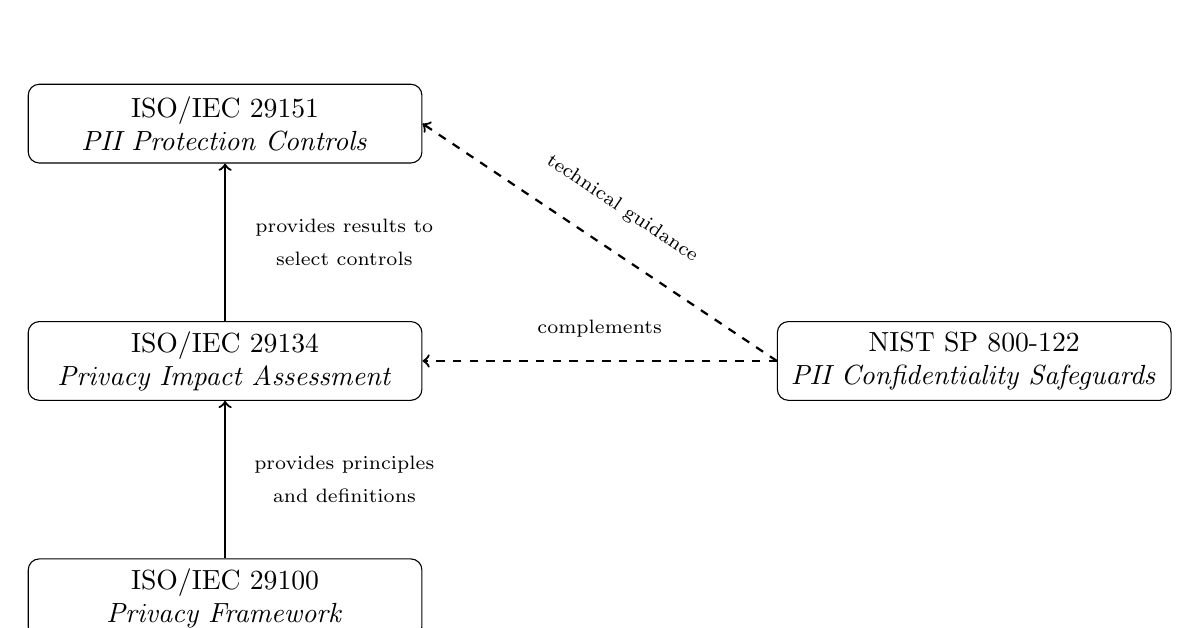
\begin{tikzpicture}[
    node distance=2cm,
    every node/.style={rectangle, draw, rounded corners, align=center, minimum width=5cm, minimum height=1cm}
]

% Nodes
\node (iso29100) {ISO/IEC 29100\\\textit{Privacy Framework}};
\node (iso29134) [above=of iso29100] {ISO/IEC 29134\\\textit{Privacy Impact Assessment}};
\node (iso29151) [above=of iso29134] {ISO/IEC 29151\\\textit{PII Protection Controls}};

\node (nist) [right=4.5cm of iso29134] {NIST SP 800-122\\\textit{PII Confidentiality Safeguards}};

% Solid arrows (ISO structure)
\draw[->, thick] (iso29100) -- node[right=-1cm, draw=none]{\scriptsize provides principles\\\scriptsize and definitions} (iso29134);
\draw[->, thick] (iso29134) --  node[right=-1cm, draw=none]{\scriptsize provides results to\\\scriptsize select controls} (iso29151);

% Dashed arrows to NIST
\draw[->, thick, dashed] (nist.west) -- node[above, sloped, draw=none]{\scriptsize technical guidance} (iso29151.east);
\draw[->, thick, dashed] (nist.west) -- node[above=-0.1cm, sloped, draw=none]{\scriptsize complements} (iso29134.east);

\end{tikzpicture}
\caption{Relationship between ISO/IEC 29100, 29134, 29151 and NIST SP 800-122}
\end{figure}

To support a better understanding and comparison, the standards are examined based on a set of common
attributes including \textbf{objectives}, \textbf{scope} and \textbf{level of abstraction} at which they operate. Other comparison criteria
include the type of \textbf{output} each standard provides, the \textbf{methodological approach} they adopt (principle-base, risk-based, control-based),
and the various \textbf{roles} and \textbf{stakeholders} they address.

\subsection{Objectives}
The first aspect to consider is the \textbf{primary objectives} of each standard. 
ISO/IEC 29100 aims to establish
a \textbf{high-level framework} for PII protection by defining a \textbf{common terminology}, identifying the \textbf{actors}
that are involved in PII processing and outlining the fundamental \textbf{principles} for privacy protection.

\vspace{\baselineskip}
ISO/IEC 29134 has a different objective, focusing on providing a \textbf{structured methodology} for conducting
Privacy Impact Assessments (PIAs) focusing on the \textbf{identification}, \textbf{evaluation} and \textbf{treatment} of privacy risks
throughout the whole lifecycle of a process or system. 

\vspace{\baselineskip}
In contrast ISO/IEC 29151 translates the high-level principles
of ISO/IEC 29100 and the risk assessment results from ISO/IEC 29134 into \textbf{specific operational controls}
that organizations can implement to protect PII.

\vspace{\baselineskip}
Finally, NIST SP 800-122 serves several purposes:
it offers a \textbf{detailed and context-driven guide} to protecting the confidentiality of PII, introducing
\textbf{impact levels}, \textbf{risk factors} and \textbf{safeguard recommandations} that organizations can apply based on their specific needs.
Although their objectives differ significantly, these standards together cover the full spectrum of privacy governance.

\subsection{Methodological Approaches}
The standards also differ significantly in their \textbf{methodological approach}. 
ISO/IEC 29100 adopts a \textbf{principle-based methodology} by establishing fundamental privacy principles
that guide organizations in their PII protection efforts \textbf{without prescribing specific processes or controls}.
This means that it provides a broad framework that organizations can adapt to their specific context.

\vspace{\baselineskip}
ISO/IEC 29134, on the other hand, employs a \textbf{risk-based approach} by defining a \textbf{step-by-step procedure}
for conducting PIAs, including the identification of stakeholders, information flows, evaluation of the threats,
impacts and likelihoods and the selection of appropriate risk treatment options. 

\vspace{\baselineskip}
ISO/IEC 29151 takes a \textbf{control-based approach}, translating privacy risks and principles
into specific \textbf{technical security and privacy controls} aligned with the ISO/IEC 27002 framework.

\vspace{\baselineskip}
NIST SP 800-122 combines both \textbf{risk-based and control-based approaches} offering 
detailed criteria for determining PII confidentiality impact levels and recommending safeguards accordingly.

\vspace{\baselineskip}
These methodological differences illustrate how the standards operate at complementary layers, conceptual,
analytical, operational and technical, within a \textbf{unified privacy management ecosystem}.

\subsection{Scope and Regulatory Context}
Another important aspect to consider is the \textbf{scope} and \textbf{regulatory context} of each standard.
The ISO/IEC 29100 series is designed for \textbf{global applicability} and is intended to be \textbf{technology and jurisdiction-neutral},
allowing organizations of any size or sector to implement its principles and guidelines for a consistent
privacy management approach worldwide.
ISO/IEC 29001, 29134 and 29151 are commonly adopted by organizations seeking to \textbf{align with international best practices}
for privacy protection, such as GDPR, CCPA or other data protection regulations.

\vspace{\baselineskip}
NIST SP 800-122, in contrast, originates within the U.S. federal context and is primarily intended for \textbf{federal agencies}
and entities that handle PII on behalf of the U.S. government. Although it is tailored to the U.S. regulatory environment,
its guidelines and risk-based reccommendations are widely adopted internationally.

\vspace{\baselineskip}
These differences highlight how ISO standards aim to support broad governance and organizational compliance \textbf{across different legal contexts},
while NIST provides detailed operational guidance tailored to a specific regulatory context yet adaptable to broader use cases.

\subsection{Integration and Complementarity}
A key aspect emerging from this comparison is that the four standars are not intended to function in isolation,
but are instead \textbf{complementary components} of a comprehensive privacy management architecture. 
ISO/IEC 29100 establishes the foundational privacy principles and terminology that guide the interpretation and application of the other standards. 

\vspace{\baselineskip}
ISO/IEC 29134 builds directly on this foundation by providing a structured methodology to assess privacy risks and determine whether and how PII processing 
may impact individuals. 

\vspace{\baselineskip}
ISO/IEC 29151 then operationalizes the output of the PIA process by defining concrete controls 
and implementation guidance tailored to the risks identified through ISO/IEC 29134 and aligned with the principles of ISO/IEC 29100. 

\vspace{\baselineskip}
NIST SP 800-122 complements this ISO ecosystem by offering detailed technical safeguards and confidentiality impact assessment criteria that organizations 
can use to strengthen both their risk evaluation and their operational controls.

\vspace{\baselineskip}
When combined, these standards provide a comprehensive and layered approach that spans conceptual governance, analytical evaluation, 
operational implementation and technical protection.

\subsection{Critical Discussion}
Taken together, the four standards reveal a \textbf{complementary balance of strengths} but also \textbf{limitations} that organizations 
should take into account when adopting them. 

\vspace{\baselineskip}
ISO/IEC 29100 and ISO/IEC 29134 are very strong in 
providing a structured governance perspective (defining principles, roles and risk assessment methodologies) but they
leave implementation choises to organizations. ISO/IEC 29151 fills this gap by providing concrete controls, but
its effectiveness depends on the quality of the underlying risk assessment process and the organization's ability
to adapt controls to their specific context. 

\vspace{\baselineskip}
NIST SP 800-122 excels for its practical orientation and detailed guidance 
on condifentiality safeguards, but its focus is narrower than that of the ISO standards and primarly centered on U.S. federal environment.

\vspace{\baselineskip}
Despite these limitations, the standards are most effective when used in combination: 
ISO provides the governance and \textbf{methodological backbone} while NIST enriches the framework with \textbf{actionable technical criteria}. 
This layered approach enables organizations to build privacy programs that are conceptually robust, risk-aware and operationally sound, 
while maintaining the flexibility needed to adapt to varying legal and technical contexts.

\begin{table}[h!]
    \centering
    % chktex-file 44
    \begin{tabular}{|>{\raggedright\arraybackslash}p{3.5cm}|
                >{\raggedright\arraybackslash}p{3.5cm}|
                >{\raggedright\arraybackslash}p{3.5cm}|
                >{\raggedright\arraybackslash}p{3.5cm}|}
    \hline
    \textbf{Dimension} &
    \textbf{ISO/IEC 29100} &
    \textbf{ISO/IEC 29134} &
    \textbf{ISO/IEC 29151} \\
    \hline

    \textbf{Primary Objective} &
    Define privacy framework, principles and roles &
    Provide methodology for Privacy Impact Assessment (PIA) &
    Define operational controls for PII protection \\ 
    \hline

    \textbf{Approach} &
    Principle-based, conceptual &
    Risk-based, methodological &
    Control-oriented, implementation-driven \\
    \hline

    \textbf{Output} &
    Privacy principles, terminology, actors &
    PIA report, risk evaluation, treatment plan &
    Set of privacy and security controls aligned with ISO/IEC 27002 \\
    \hline

    \textbf{Scope of Application} &
    All organizations processing PII &
    Projects, systems or processes involving PII &
    Organizations implementing operational privacy safeguards \\
    \hline

    \textbf{Role in Privacy Management} &
    Foundational layer: defines “what” privacy requires &
    Analytical layer: evaluates “how” PII processing affects individuals &
    Operational layer: defines “how” risks must be mitigated \\
    \hline
    \end{tabular}

\vspace{0.5cm}

\renewcommand{\arraystretch}{1.4}
\begin{tabular}{|>{\raggedright\arraybackslash}p{3.5cm}|p{10.5cm}|}
\hline
\textbf{NIST SP 800-122} &
Provides technical guidance for protecting the confidentiality of PII, defining impact levels, risk factors and recommended safeguards. Complements ISO 29134 and ISO 29151 with detailed technical criteria. \\
\hline
\end{tabular}

\caption{Comparative overview of ISO/IEC 29100, 29134, 29151 and NIST SP 800-122}
\end{table}

\clearpage

% Section 6: Conclusion
\section{Conclusion}\label{sec:conclusion}
The study conducted in this report shows how modern privacy governance and 
management cannot rely on a single standard or framework but must instead
be built upon a \textbf{combination of multiple guidelines, controls and assessment 
practices}. While each single standard analyzed approaches privacy from a different
perspective, the broader view that emerges highlights the importance for organizations
to adopt a structured, risk-aware and priciple-based framework capable
of adapting to evolving regulatory requirements and technological advancements.

\vspace{\baselineskip}
From this work it is clear that privacy protection nowadays is not just 
a matter of technical measures or compliance checklists, but requires
a \textbf{continuous alignment} between organizational governance, risk evaluation, 
security controls and and accountability mechanisms. The combination of conceptual
frameworks, operational guidelines, implementation controls and context-specific
technical guidance provides organizations with the depth needed to build
privacy-by-desing systems that \textbf{remain effective across different scenarios}.

\vspace{\baselineskip}
This project also highlights how privacy standards are converging toward \textbf{shared 
principles} such as data minimization, accountability and security, yet remaining
flexbile enough to be tailored to different regulatory ecosystems. This \textbf{interplay 
between consistency and adaptability} is essential for organizations 
operating across jurisdictions or relying on emerging technologies 
such as cloud services, AI-driven processing and large-scale data analytics.

\vspace{\baselineskip}
Looking ahead, it is evident that the increasing complexity of data ecosystems
suggests that privacy will continue to evolve toward \textbf{greater integration}
with cybersecurity frameworks, automated risk assessment tools and continuous
monitorin practices. Organizations will not only need to select the most
appropriate standards, but also to cultivate interal expertise capable of
interpreting them \textbf{dinamically}.

\vspace{\baselineskip}
Finally, this report demonstrates that the strength of a privacy program
lies not just in the \textbf{adoption of specific standards}, but in the \textbf{coherent 
orchestration of complementary standards}. When used togheter, the frameworks
analyzed in this report enable organizations to transform privacy from 
a compliace requirement into a \textbf{sustainable and strategic asset}.
\clearpage

% Bibliography
\nocite{*}
\bibliographystyle{plain} % puoi cambiare in alpha, ieee, apa, ecc.
\bibliography{references}


\end{document}
